\documentclass[mathematics,article,accept,pdftex,moreauthors]{Definitions/mdpi}
%\documentclass[preprints,article,submit,pdftex,moreauthors]{Definitions/mdpi}
% For posting an early version of this manuscript as a preprint, you may use "preprints" as the journal. Changing "submit" to "accept" before posting will remove line numbers.

%----------
% submit
%----------
% The class option "submit" will be changed to "accept" by the Editorial Office when the paper is accepted.

%=================================================================
% MDPI internal commands - do not modify
\firstpage{1} 
\makeatletter 
\setcounter{page}{\@firstpage} 
\makeatother
\pubvolume{1}
\issuenum{1}
\articlenumber{0}
\pubyear{2026}
\copyrightyear{2026}
\externaleditor{Firstname Lastname} % More than 1 editor, please add `` and '' before the last editor name
\datereceived{18 March 2026} 
\daterevised{10 April 2026} % Comment out if no revised date
\dateaccepted{14 April 2026} 
\datepublished{ } 
%\datecorrected{} % For corrected papers: "Corrected: XXX" date in the original paper.
%\dateretracted{} % For retracted papers: "Retracted: XXX" date in the original paper.
%\doinum{} % Used for some special journals, like molbank
%\pdfoutput=1 % Uncommented for upload to arXiv.org
%\CorrStatement{yes}  % For updates
%\longauthorlist{yes} % For many authors that exceed the left citation part
%\IsAssociation{yes} % For association journals

%=================================================================
% Add packages and commands here. The following packages are loaded in our class file: fontenc, inputenc, calc, indentfirst, fancyhdr, graphicx, epstopdf, lastpage, ifthen, float, amsmath, amssymb, lineno, setspace, enumitem, mathpazo, booktabs, titlesec, etoolbox, tabto, xcolor, colortbl, soul, multirow, microtype, tikz, totcount, changepage, attrib, upgreek, array, tabularx, pbox, ragged2e, tocloft, marginnote, marginfix, enotez, amsthm, natbib, hyperref, cleveref, scrextend, url, geometry, newfloat, caption, draftwatermark, seqsplit
% cleveref: load \crefname definitions after \begin{document}
	\usepackage[algo2e,linesnumbered,ruled]{algorithm2e} 
	\usepackage{tabularx}       % automatic column width
	\usepackage{mathtools}  
	\usepackage{amsfonts}       % mathbb
	\usepackage{xfrac}          % slanted fractions
	\usepackage{bm}             % bold greeks 
	\usepackage{setspace}       % for controlled interline
	\usepackage{graphicx}
	\usepackage{amsmath}        % multiline formulas
	\usepackage{array}          % for better column control
	\usepackage{xcolor}         % for coloring blocks of text
	\usepackage{rotating} 	
	\usepackage{soul}
   \newcommand{\highlight}[1]{\textcolor{blue}{#1}}

%=================================================================
% Full title of the paper (Capitalized)
\Title{Optimal Partitioning Changepoint Analysis}

%\newcommand{\rev}[1]{{\color{blue}#1}}
% Author Orchid ID: enter ID or remove command
\newcommand{\orcidauthorA}{0000-0002-1220-1235} % Add \orcidA{} behind the author's name
\newcommand{\orcidauthorB}{0009-0004-0388-4988} % Add \orcidB{} behind the author's name

% Authors, for the paper (add full first names)
\Author{Vittorio %MDPI: Please carefully check the accuracy of names and affiliations.
 Maniezzo $^{1,}$*%MDPI: Newly added * information of the correspondence authors. Please confirm.
\orcidA{} and Lisa Vecchi $^{1}$\orcidB{}}

%\longauthorlist{yes}

% MDPI internal command: Authors, for metadata in PDF
\AuthorNames{Vittorio Maniezzo and Lisa Vecchi}

% Affiliations / Addresses (Add [1] after \address if there is only one affiliation.)
\address{%
	$^{1}$ \quad Department of Computer Science, University of Bologna, 40126 Bologna%MDPI: Newly added  information. Please confirm.
, Italy\\
	%$^{2}$ \quad University %MDPI: The department/school/faculty/campus of this university is required. Please try to provide this information.
 %of \hl{Bologna}%MDPI: If affiliation 1/2 are same, if so, please merge them.
%, 40126 Bologna, Italy; lisa.vecchi@studio.unibo.it\\
	}

% Contact information of the corresponding author
\corres{Correspondence: vittorio.maniezzo@unibo.it}

% Abstract (Do not insert blank lines, i.e.,~\\)
\abstract{Detecting changepoints in time series is a fundamental task in statistical modeling and data-driven decision-making. We introduce a novel set partitioning-based model for changepoint detection that leverages combinatorial optimization to identify an optimal set of segments explaining the observed data.
Unlike conventional dynamic programming approaches, which rely on restrictive structural assumptions on the cost function to ensure tractability, our formulation is based on Integer Linear Programming. While the standard additivity assumption on segment-wise costs is retained, the proposed framework departs from existing methods in its ability to incorporate both local and global structural constraints directly within the optimization model. In particular, it supports a broad class of constraints, ranging from simple segment-level restrictions to complex global conditions coupling multiple segments, without requiring modifications to the underlying solution scheme. This enhanced modeling capability constitutes the main contribution of the work, significantly increasing the expressiveness of the framework while preserving the tractability of additive cost structures.
The model’s design enables high adaptability to different application domains, including finance, bioinformatics, and industrial monitoring.
The efficiency of modern MILP solvers, combined with tailored dominance rules, enables the solution of instances with several hundreds of observations in practical time. Computational results indicate that the approach extends tractability beyond previously studied settings, effectively handling classes of instances whose structural constraints could not be accommodated by existing methods, while retaining robustness and interpretability.}

% Keywords
\keyword{time series; set partitioning problem; segmentation; changepoint detection}

% The fields PACS, MSC, and JEL may be left empty or commented out if not applicable
%\PACS{J0101}
\MSC{62M10,90C10,90C11}
%\JEL{}

\begin{document}
%%%%%%%%%%%%%%%%%%%%%%%%%%%%%%%%%%%%%%%%%%
\section{Introduction} %MDPI: Please check all equipment and software in this text (if used): 1. Please state the name of the manufacturer, city, state abbreviation (for USA and Canada only) and country from where the equipment was sourced. This applies to all first instances of each mentioned piece of equipment in the manuscript. e.g., Bravo Liquid Handler (Agilent Technologies Inc., Santa Clara, CA, USA); 2. Please state the version number of software used in the study. If a version is not available, please provide a valid link to the software's website instead and state the access date (day, month and year). This applies to the first instance of each mentioned software in the manuscript. E.g., MATLAB (v2024).
\label{sec:intro}

Changepoint detection (CPD) is the task of identifying abrupt changes in the statistical properties of a time series and constitutes a foundational problem across statistics, machine learning, and~signal processing~\cite{LMS14,AC17,TOV20}. The~objective of CPD is to partition a temporal sequence into contiguous, non-overlapping segments, each characterized by internally homogeneous behavior. Such segmentation enables a clearer understanding of the underlying data-generating process and facilitates the application of targeted analytical or predictive models at the segment level. As~a result, effective changepoint detection plays a critical role not only in descriptive analysis, but~also in forecasting, anomaly detection, and~data-driven~decision-making.

CPD assumes a pivotal function in a wide range of application domains, including financial market analysis (regime shifts), industrial process monitoring (fault detection), climate science (trend changes), and~bioinformatics (genomic variation analysis). Across these domains, a~CPD method must satisfy two key requirements: (i) accurately segment data so as to faithfully represent the underlying process, and~(ii) provide a globally optimal solution, since suboptimal segmentation can propagate errors downstream and lead to significant real-world~costs.

Time series segmentation has therefore attracted extensive attention, leading to the development of a broad spectrum of methodologies, including classical statistical techniques, Bayesian approaches, machine learning algorithms, and~hybrid models. Among~these, segmentation based on linear models remains particularly prominent due to its computational efficiency and interpretability. This setting, commonly referred to as {\it piecewise linear regression}%MDPI: Please confirm if the italics are necessary; if not, please remove them. The following highlights are the same.
~\cite{KCHP02}, assumes that the time series can be approximated by a sequence of linear trends, each corresponding to a distinct~segment. 

For exact and globally optimal changepoint detection under additive cost structures, the~dominant methodological paradigm is dynamic programming (DP). Methods such as Optimal Partitioning exploit the recursive structure of the problem, constructing the optimal segmentation for a sequence of length $n$ from optimal solutions to shorter prefixes. This approach yields polynomial-time algorithms under suitable assumptions and has proven highly effective in practice. However, the~effectiveness of the DP framework fundamentally relies  on the additive decomposability of segment-wise costs, typically combined with a penalty proportional to the number of segments. Accelerated variants additionally require regularity conditions on the cost function, which can be interpreted as a superadditivity-type inequality, to~justify~pruning.

This additive and recursive structure imposes a significant modeling limitation. In~many practical settings, the~analyst wishes to enforce global structural constraints that couple properties of all selected segments. Examples include limiting the total duration of short segments, bounding the number of changepoints within specific time windows, or~enforcing regularity in segment lengths to avoid excessively fragmented solutions. While certain such constraints can, in~principle, be approximated through state augmentation or penalty tuning, doing so rapidly compromises the tractability and scalability of DP-based methods. As~a result, DP frameworks remain largely confined to locally additive objectives, restricting their applicability in scenarios where global control over the segmentation structure is~essential.

To overcome this limitation, we propose a novel formulation of the CPD problem as a combinatorial optimization model, specifically a set partitioning problem, possibly extended to its set covering relaxation. In~this formulation, all feasible segments are pre-enumerated and treated as decision variables, and~changepoint detection reduces to selecting a minimum-cost subset of segments that exactly covers the time series. Unlike breakpoint-indicator or network-flow formulations, this representation models segments as atomic objects, thereby naturally supporting richer interactions and more expressive global~constraints.
 
{The relaxation of the set partitioning formulation to a set covering problem relinquishes the exactness guarantee: the resulting solution is heuristic in nature because overlapping runs must be resolved through postprocessing. Although~this compromise yields significant computational gains, it should not be conflated with the global optimality guaranteed by the exact TSSP formulation.}

{The key advantage of the MILP framework lies not only in its ability to reproduce the classical additive cost structure, but,~more importantly, in its capacity to enforce complex global constraints through simple linear (in)equalities. These constraints can link arbitrary subsets of segment variables, control aggregate properties such as the number, length, or~distribution of segments, and~encode domain-specific structural requirements that are difficult or impractical to express within DP-based models. More specifically, while DP-based approaches can naturally accommodate local segment-level constraints, such as minimum segment length, slope bounds, and~admissible breakpoint positions, incorporating  global constraints that couple properties across the entire segmentation typically leads to an substantial growth of the state space, making such  extensions computationally impractical. Unlike breakpoint-indicator or network-flow formulations, the~proposed set partitioning approach provides a direct and flexible mechanism for global control over the segmentation. While MILP solving is NP-hard in general, recent advances in solver technology, together with problem-specific preprocessing and bounding techniques, make this approach computationally viable for problem sizes of practical interest. }
In this paper, we introduce Set-Partitioning based Changepoint Detection (SP-CPD) as a framework for optimal time series segmentation. Our main contributions are as follows:

A set-partitioning MILP formulation with additional constraints for CPD with global structural control.
We formulate the changepoint detection problem as a set partitioning model, enabling the direct incorporation of global constraints that are beyond the practical reach of dynamic programming~methods.

\textls[-15]{Enhanced modeling fidelity through global constraints:
We demonstrate the practical value of the proposed framework by introducing and analyzing several global constraints that improve the interpretability, robustness, and~domain relevance of the resulting~segmentations.}

%Scalability through preprocessing and dominance rules.
%We develop specialized preprocessing techniques, including dominance rules and bounding strategies, that significantly reduce the number of candidate segments and allow the model to scale to time series with several thousand observations.

Competitive computational performance and solution quality.
Through extensive computational experiments, we show that SP-CPD produces higher-quality segmentations while achieving runtimes that, up~to mid-sized series, are comparable to state-of-the-art DP-based and heuristic~methods.

The paper further illustrates the versatility of the proposed approach through a range of real-world applications, including financial time series, epidemiological data, and~environmental monitoring. Common challenges such as noise, high variances, and~non-stationarity are included, highlighting the advantages of MIP-based changepoint detection in addressing domain-specific structural~requirements.

\textls[-15]{The remainder of this paper is organized as follows. Section~\ref{sec:literature} reviews the relevant literature. Section~\ref{sec:SCPmodel} presents the proposed set partitioning model. Section~\ref{sec:computation} reports the computational results. Finally, Section~\ref{sec:conclusions} concludes and outlines directions for future~research.}

\section{Related~Literature} 					\label{sec:literature}
The problem of optimal changepoint detection and time series segmentation has been extensively studied, and~a wide range of exact and approximate methods have been proposed. Comprehensive surveys are provided in~\cite{AC17,TOV20}, which classify approaches into statistical, Bayesian, algorithmic, and~learning-based families. In~this section, we focus specifically on exact optimization-based formulations for changepoint detection and highlight their modeling assumptions and limitations relative to the proposed~approach.

Dynamic programming (DP) constitutes the dominant paradigm for exact changepoint detection under additive cost structures. Classical methods such as Segment Neighborhood~\cite{AL89} and Optimal Partitioning~\cite{JSB05} formulate the problem as the minimization of a sum of segment-wise losses plus a penalty on the number of changepoints. By~exploiting the optimal substructure of the problem, these methods guarantee global optimality and admit polynomial-time algorithms under suitable~assumptions.

Substantial effort has been devoted to improving the practical efficiency of DP-based CPD. Notable examples include the Pruned Exact Linear Time (PELT) algorithm~\cite{KFE12}, which uses inequality-based pruning to reduce the search space, and~functional pruning approaches~\cite{R10,J13}, which exploit convexity properties of the segment cost. These methods have become state of the art for large-scale problems with additive~objectives.

Despite their efficiency, DP-based models fundamentally rely on the separability of the objective function across segments. This reliance severely limits their ability to incorporate constraints that couple decisions across the entire segmentation. While constrained DP and state-augmented formulations have been proposed for specific problems~\cite{HRFB13}, the~resulting state spaces typically grow exponentially, making such approaches impractical beyond very limited forms of global control. Consequently, DP methods remain best suited for problems with simple additive objectives and limited structural~constraints.

Several optimal CPD models reinterpret the segmentation problem as a shortest-path problem on a directed acyclic graph, where nodes correspond to time indices and arcs represent feasible segments weighted by their associated costs~\cite{B61,PC75}. This representation is then solved by DP models that yield efficient shortest-path~algorithms.

Although graph-based formulations offer valuable conceptual insight and algorithmic flexibility, they inherit the same structural limitations as the DP at their core. In~particular, it is difficult to express global constraints that do not decompose additively along a path without introducing additional dimensions or complex side constraints, which compromise tractability once~again.

Mixed-Integer Programming (MIP) has been previously applied to changepoint detection and piecewise regression, primarily through formulations based on breakpoint indicator variables or segment assignment variables. Early work on segmented regression using integer programming can be traced back to~\cite{H66,F58}, with~more recent formulations incorporating modern MIP solvers for exact piecewise linear fitting~\cite{BKM16}, while a recent quadratic formulation based on big-M constraints can be found in~\cite{PRSS25}.

In breakpoint-based formulations, binary variables indicate whether a changepoint occurs at a given time index, while continuous variables model segment-specific parameters. These models allow for regression and segmentation decisions to be optimized jointly and can accommodate certain side constraints. However, constraints involving segment-level properties—such as length distributions, aggregate statistics of selected segments, or~interactions between non-adjacent segments—typically require additional auxiliary variables and complex logical constraints, leading to weak linear relaxations and limited scalability.
Assignment-based formulations, in~which observations are assigned to segments via binary variables, suffer similar difficulties when enforcing contiguity and global structural constraints. In~both cases, segmentation is encoded implicitly, rather than directly treating segments as decision~objects.

The approach proposed in this paper differs fundamentally from the above paradigms by adopting a set-based perspective. Each feasible segment is explicitly represented as a decision variable, and~the segmentation problem is formulated as a set partitioning (or covering) problem in which the time axis must be covered (at least) once. While set covering and set partitioning models are classical tools in combinatorial optimization~\cite{B69,S03}, they have received comparatively little attention in the changepoint detection~literature.

By associating segments with decision variables, the~set-partitioning formulation provides a natural mechanism for expressing global structural constraints directly at the segment level. Aggregate constraints on the number, length, distribution, or~interaction of segments can be imposed through simple linear inequalities, without~resorting to state augmentation or intricate logical constructs. This distinguishes the proposed SP-CPD framework from existing MIP formulations and enables a level of modeling expressiveness that is difficult to achieve within DP-based, shortest-path, or~breakpoint-indicator~models.

In summary, existing optimal CPD models exhibit a clear trade-off between computational efficiency and modeling flexibility. Dynamic programming and graph-based approaches provide excellent performance for additive objectives, but offer limited support for global structural constraints. Prior MIP formulations increase modeling power, but typically encode segmentation implicitly and encounter scalability issues when complex segment-level constraints are~introduced.

The proposed SP-CPD framework occupies a complementary position in this landscape. By~combining a set-partitioning formulation with modern MILP techniques and problem-specific preprocessing, it delivers global optimality while substantially expanding the class of constraints that can be handled in a principled and scalable manner. This positions SP-CPD as a flexible and extensible optimization framework for changepoint detection in applications where global structure and domain-specific requirements play a central~role.

{Finally, it is worth clarifying the scope of the proposed framework with respect to forecasting. The~SP-CPD model, as~well as the DP-based methods reviewed in this section, rely on piecewise linear interpolation to fit segments to the observed data. As~a consequence, these approaches are inherently descriptive and suited for structural modeling purposes only: they characterize the historical behavior of the series, but do not provide a mechanism for out-of-sample prediction. Out-of-sample forecasting requires dedicated time series models that  explicitly account for temporal dependencies and autocorrelation structures, such as ARMA or ARIMA models~\cite{box2015,hyndman2018}. The~proposed changepoint detection framework should therefore be understood as a segmentation and structural modeling tool, complementary to but distinct from forecasting methodologies~\cite{lopez2021}.}

\section{Extended Set Partitioning and Covering~Models}  \label{sec:SCPmodel}
The CPD problem can be naturally modeled from a set partitioning perspective: all subsequences satisfying predefined structural properties—termed feasible runs—are generated and scored according to a segment-specific quality metric under~an additivity assumption on the cost function. The~segmentation problem is then formulated as the selection of a collection of runs that partitions the time index set while optimizing a global objective based on residual loss or model fit. The~resulting formulation is a 0–1 integer linear program, which can be viewed as a special case of a mixed-integer linear program (MILP), thereby allowing for the use of state-of-the-art MILP solvers~\cite{FLS09}. This framework provides considerable flexibility, as~additional modeling requirements can be seamlessly encoded via linear~constraints.

A Set Partitioning Problem (SPP) lies at the core of the formulation. The~objective is to minimize an aggregate residual-based cost, while the constraints enforce that each time index of the series is covered exactly once by the selected segments. No restriction is imposed on the functional form of the segment model: it may consist of linear regression (yielding piecewise linear regression), but~also of nonlinear or nonparametric specifications. Moreover, different runs may be associated with different model classes without altering the structure of the optimization~problem.

Formally, let $X = [x_j]$, $j = 1,\ldots,nruns$, denote the binary decision variables, where $x_j = 1$ if run $j$ is selected and $x_j = 0$ otherwise. Feasible runs may be generated so as to incorporate preliminary dominance rules by, for~instance, excluding segments that are too short or too long. Each run $j$ is assigned a cost $c_j$, computed according to any suitable goodness-of-fit or loss metric proposed in the literature, including $R^2$, SER, $\chi^2$, RMSE, variance-based criteria, etc. The~partitioning/covering constraints ensure that every series point is included in (exactly) one selected~run.

The resulting Time Series Set Partitioning (TSSP) model is defined as follows. Let \linebreak  $a_{ij} \in \{0,1\}$ \textls[15]{be a coefficient equal to 1 if and only if run $j$ covers time index $i$, for} \linebreak  $i = 1,\ldots,npoints$ and $j = 1,\ldots,nruns$. In~formulation TSSP, we also included a constraint on the cardinality of the solution~set. %MDPI: 1. Please recheck all equations and make sure there are no duplicated independent equations in the whole manuscript. Thanks! 2. The variables in the equations should be consistent with the main text. Please double-check and Please ensure all variables/values in the equation appear in the same format in the text (normal/italic/bold/subscript/superscript).

\begin{alignat}{4}
	(TSSP) \hspace{0.5cm} z_{TSSC} = \min &\; \sum_{j=1}^{nruns} c_j x_{j}  \label{eq:SCPobj} \\
	s.t. &\; \sum_{j=1}^{nruns}a_{ij}x_{j} = 1, & \hspace{1.5cm} i=1,\dots,npoints  \label{eq:SCPcov} \\
	&\; \sum_{j=1}^{nruns} x_{j} \leq maxruns \label{eq:SPPext}\\
	&\; x_j \in \{0,1\}, &\; j=1,\dots,nruns  \label{eq:SCPvar}
\end{alignat}

Additional variables can be included in the model associating them with the $X$ decision variables; for~example, it is possible to associate the starting time $s_i$, the~end time $e_i$ with each variable $x_i \in X$. While redundant in this formulation, they might become important to express the constraints listed in Section~\ref{subsec:additional_constraints}.

Unfortunately, in~real-world applications, the number of feasible runs can be very large, making the resulting SPP computationally demanding and, in~some cases, intractable within acceptable time limits. From~a polyhedral perspective, the~set partitioning formulation is typically tighter, but also harder to explore computationally, as~the equality constraints induce a more restrictive feasible region and a combinatorially demanding branching structure. To~mitigate this issue, we can relax the equality constraints (\ref{eq:SPPext}) into inequalities, thereby transforming the formulation into a Set Covering Problem (SCP). The~covering polyhedron is generally easier to handle algorithmically and can be solved in significantly larger dimensions, albeit with a weaker linear programming~relaxation. 

{The SCP relaxation allows for multiple runs to cover the same series points, and~therefore a postprocessing phase is required to extract a feasible segmentation from the (possibly overlapping) covering solution. As~a result, the~solution produced by the TSSC model is heuristic: global optimality is no longer guaranteed, and the final segmentation is obtained through a  greedy fixing procedure. The~resulting set covering formulation is denoted by~TSSC.}

State-of-the-art MIP solvers are highly effective on SCP formulations; however, very large instances may still entail substantial computational effort. To~further enhance scalability, ref.~\cite{M24} proposed a Lagrangian matheuristic~\cite{the_book} for the TSSC problem where  all covering constraints (\ref{eq:SCPcov}) are relaxed by associating a Lagrangian multiplier $\lambda_i$ with each constraint, $1 \leq i \leq npoints$, while retaining only the relaxed covering constraint in the formulation. 
The resulting Lagrangian model is solved via a subgradient optimization scheme. The~corresponding Lagrangian subproblem is computationally simple: at each iteration, it amounts to selecting at most the $maxruns$ variables with the most negative reduced costs. A~simple fixing heuristic is embedded within the procedure: the incumbent solution of the subproblem, which may be infeasible with respect to the relaxed covering constraints, is iteratively augmented by adding selected variables until feasibility is restored. This relaxation makes it possible to easily include constraints such as the maximum number of segments allowed. However, in~most cases, additional constraints must be added to the subproblem or relaxed themselves, which makes the approach~impractical.

In any case, after~solving a set covering relaxation, postprocessing is required to transform any SCP solution into a feasible SPP segmentation. This can be accomplished in linear time by scanning each region of overlapping runs and identifying the splitting point that minimizes the total cost obtained by assigning the preceding observations to the preceding segment and the subsequent observations to the following~segment.

\subsection{Cost~Function}	\label{subsec:costfunc}

Models TSSP and TSSC are suitable for offline (or anytime) analysis assuming additive costs. The~model is independent on the specific function used to quantify the cost associated with each segment. The~CPD literature proposes different cost functions, including negative log-likelihood (\cite{H93}) and quadratic loss or cumulative sums (\cite{IT94}), but~any statistical measure of fit can be used for the task. Each measure favors different characteristics of the model, and the results can be widely~different.

In practical applications of CPD, model quality is often judged less by its formal optimality properties and more by the interpretability of the resulting segmentation. In~many real-world settings, the~most useful segmentation is not necessarily the one that minimizes a given objective function, but~rather the one that aligns with human perception of structural changes or provides a coherent narrative for subsequent decision-making. Accordingly, the~utility of a cost function may depend as much on the clarity and explanatory power of its segmentation as on its predictive~accuracy.

To reconcile algorithmic outputs with visual or domain-based expectations, many selection procedures incorporate penalty terms that regulate the number of detected changepoints. These penalizations effectively allow practitioners to adjust the segmentation to better match subjective expectations. However, the~resulting models should be regarded as practically useful approximations rather than representations of an underlying “true” model, which is unlikely to be included among the finite set of candidate models considered in practice %MDPI: Newly added citation link. Please confirm.
~\cite{HRFB13}.

A further limitation of user-defined penalization schemes is that they implicitly require human feedback. In~heterogeneous datasets, appropriate penalty calibration often needs to be tailored on a per-series basis, which limits scalability and automation. To~reduce this dependency on manual tuning, we evaluated several alternative cost functions drawn from both information-theoretic and optimization-based frameworks, with~the aim of identifying a more robust and resilient formulation suitable for automated CPD~analysis.

We evaluated a broad range of cost functions, including AIC, BIC, Chi-square statistics, MSE, QRMSE, $R^2$, RMSE, SER, and~simple variance; comparative visual results on a standard benchmark instance are represented in Figure~\ref{fig:costfunctions}. No single criterion consistently dominates the others across all benchmark instances. Performance varies depending on the underlying signal structure, noise characteristics, and~segment length distribution, supporting the claim that cost-function performance is inherently~context-dependent.

For the subsequent analysis, we focus on two representative and complementary criteria: AIC and QRMSE. AIC is well established in the CPD literature, particularly through its equivalence to penalized negative log-likelihood formulations, and~provides a theoretically grounded likelihood-based~benchmark.

QRMSE (Quarter-root-RMSE) \cite{M24}, by~contrast, lies between MSE and RMSE in terms of segment-length sensitivity. Relative to MSE, it places less emphasis on short segments, while avoiding the stronger preference for long segments induced by RMSE. This intermediate behavior makes it attractive in applications where neither aggressive segmentation nor excessive smoothing is desirable.
Specifically, QRMSE is obtained from the residual sum of squares~as

$$
QRMSE = \sqrt{\frac{SSE}{\sqrt{n}}}
$$

This %MDPI: We have added indents to paragraphs with capital letters, please confirm and check through the whole text
formulation reduces the implicit penalty associated with long segments compared with classical RMSE- or MSE-based criteria. 
As a consequence, longer segments are penalized less strongly and the resulting segmentations tend to be~smoother.



\begin{figure}[H]
	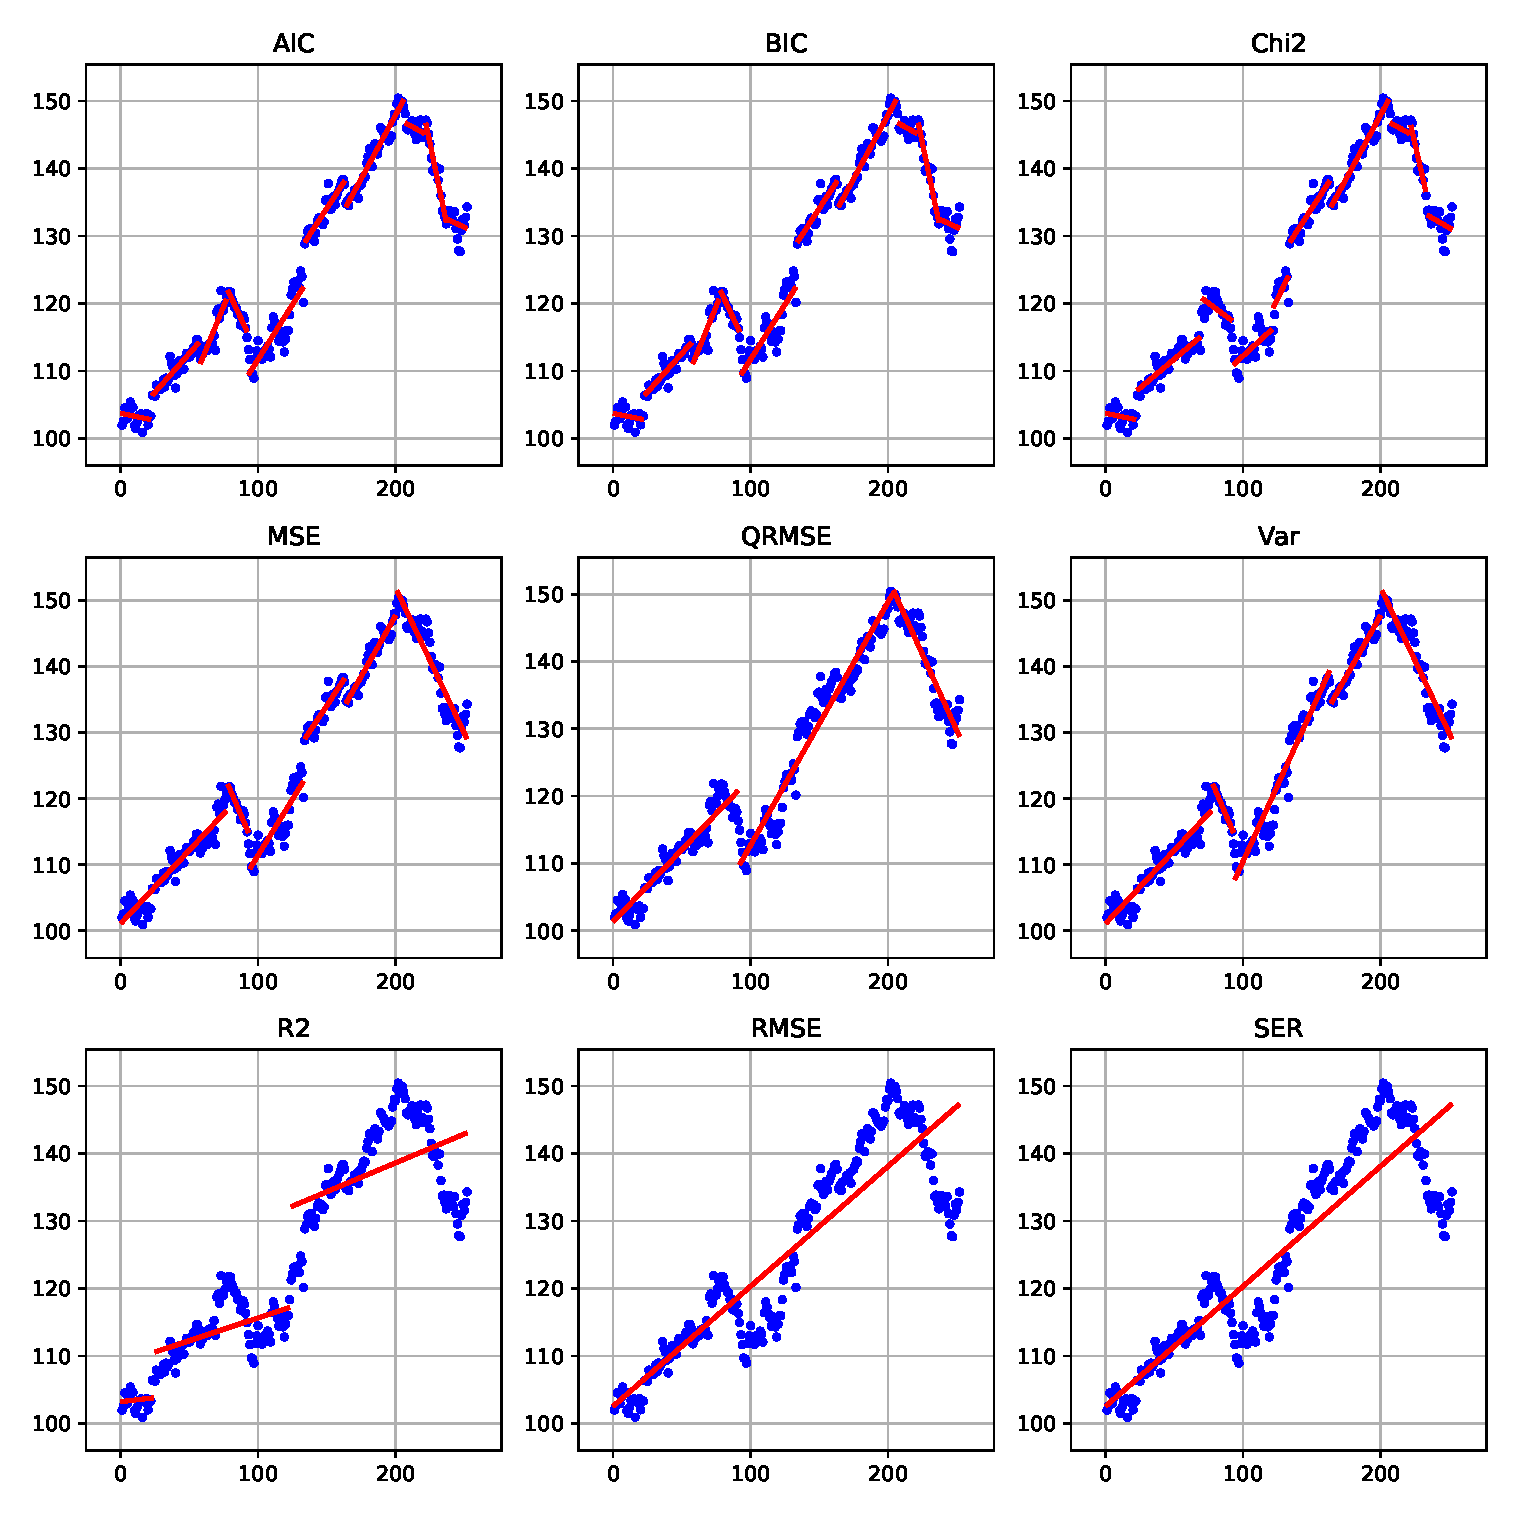
\includegraphics[width=0.99\linewidth]{ROST_global}
	\caption{Alternative %MDPI: 1. Please note that the size/White space margin of figures will be adjusted appropriately to ensure the clarity and readability of the image, Changes to the position of figures and tables may occur during the production stage. 2. Please double check all figures, if there are special color/special symbol... need add explanation in the figure caption.
 cost functions on series ROST of benchmark~M6.}
	\label{fig:costfunctions}
\end{figure}

Importantly, although~QRMSE is additive across segments and can therefore be used within optimal partitioning frameworks, it does not satisfy the inequality condition required for pruning in algorithms such as PELT. In~particular, the~cost of a merged segment may be lower than the sum of the costs of two adjacent subsegments. This violation prevents the use of the pruning guarantees that underpin the computational efficiency of such methods, limiting the practical applicability of QRMSE in large-scale~settings.

\subsection{Additional~Constraints}  \label{subsec:additional_constraints}

In many real-world applications, the~analyst is not only interested in minimizing a fitting error, but~also in enforcing interpretable and domain-driven properties on the resulting segmentation.
Many changepoint frameworks encode these ideas via global penalization rather than hard constraints—using penalties on the number of changepoints ({\it L0}), total variation ({\it L1}), or~graph-structured transitions that enforce sign alternation or monotone regimes across the entire sequence. These approaches provide a way to control global behaviors, such as roughness or regime structure, and~are usually implemented by dynamic programming or a specialized algorithm limiting the possibility to flexibly expand the proposed~model.

These are the constraints that ``operate over the whole segmentation'' and are discussed in the global constraint catalogs and changepoint detection literature (Beldiceanu, Régin; O'Hearn; Gionis; Killick; etc.), as~well as in application papers spanning different areas, including bioinformatics, econometerics, and signal processing, among~others. 

Let $\mathcal{I} = {1, \ldots, nruns}$ be the index set of feasible segments, where each segment is associated with its start and end indices $(s_i,e_i)$, $i \in I$, with~length $\ell_i = e_i - s_i + 1$, slope $\beta_i$ (in the case of linear regression), fitting cost $c_i$ and endpoint values $(v^1_i,v^2_i)$. 

For the sake of our discussion, it is important to distinguish between two classes of constraints: those that affect the feasibility of individual segments independently of the remainder of the sequence, and~those that impose conditions on the sequence as a whole. Constraints in the first class can be naturally incorporated into the segment generation process and are readily accommodated within dynamic programming frameworks. In~contrast, constraints in the second class require the introduction of additional state variables to track global properties, thereby increasing the computational burden of dynamic programming~approaches.

\subsubsection{Local Segment~Constraints} \label{subsubsec:segment_level_constraint}

Segment-level constraints restrict the admissible properties of each segment independently of the rest of the segmentation. These constraints can be implemented in the data generation phase, do not require additions to formulations TSSP or TSSC, and are easily included in DP approaches. 
Typical segment-level constraints~include:
\begin{itemize}
	\item {\it Minimum and maximum segment length: %MDPI: Please confirm if the italics are necessary; if not, please remove them. The following highlights are the same.
}	Bounds on the length of each segment (minimum spacing between changepoints) prevent over-fragmentation and excessively long segments In optimal partitioning approaches,  minimum segment size constraints can be naturally incorporated. For~instance, the~PELT algorithm~\cite{KFE12} allows for restricting the set of admissible segmentations by enforcing a lower bound on segment length and also by limiting admissible segment endpoints according to a predefined minimum segment size. This constraint is expressed as
\begin{equation}
		\ell_{\min} \leq e_i - s_i + 1 \leq \ell_{\max} \qquad i \in \mathcal{I}
	\end{equation}
	
	\item {\it Slope constraints:}
	When segments are modeled via linear regression, constraints can be imposed on segment-specific parameters, such as the slope $\beta_i$. More generally, constrained changepoint detection under affine inequality restrictions between segment parameters has been studied~\cite{hocking2017constrained}. Typical examples include bounded slopes or~directional constraints enforcing locally non-decreasing or non-increasing behavior.
\begin{equation}
		|\beta_i| \leq \beta_{\max} \qquad i \in \mathcal{I}
	\end{equation}
	 
	\item {\it Boundary exclusion:}
	Changepoints can be disallowed in the first and last $K$ observations of the series to ensure stable parameter estimation. This can be enforced by restricting admissible start and end indices:
\begin{equation}
		s_i \geq K + 1 \quad \text{and} \quad e_i \leq n - K  \qquad i \in \mathcal{I}
	\end{equation}
	where $n$ denotes the length of the~series.
	
	\item {\it Admissible breakpoint positions:}
	Changepoints may be restricted to a predefined set $\mathcal{A} \subseteq \mathcal{I}$ of admissible positions, such as calendar or seasonal markers. For~example, in~the Ruptures framework~\cite{TOV20}, the~jump parameter enforces that changepoints can only be selected on a subsampled grid of indices, effectively reducing the admissible set of breakpoint locations. In~this case, segment boundaries must satisfy
\begin{equation}
		s_i,e_i \in \mathcal{A}.
	\end{equation}
	These restrictions are useful both for computational efficiency and for incorporating prior structural information into the segmentation model. 	
\end{itemize}

\subsubsection{Global Series~Constraints} \label{subsubsec:global_series_constraints}

In contrast to segment-level constraints, global series constraints impose conditions that couple multiple segments and operate on the segmentation as a whole. 
Mixed-Integer Programming formulations can support several types of constraints belonging to this class through possibly linear inequalities linking multiple segment-selection~variables.

A list of global constraints reported in the literature is presented below. We note that several of these constraint classes generate a number of constraints that grows superlinearly with the number of feasible segments (often quadratically in practice). Explicitly including all such constraints in the model is therefore impractical. Instead, we anticipate incorporating them via a cutting-plane strategy: constraints are added on demand as violated cuts because their separation can be performed efficiently for the constraint types~considered.

\begin{itemize}
	\item {\it Global bound on the number of segments:}
	A global bound on the number of selected segments controls the overall model complexity. This constraint can be written as
\begin{equation}
		\sum_i x_i \le n_{\max}.
	\end{equation}
	Constrained dynamic programming algorithms under this setting are discussed in~\cite{hocking2017constrained}.
	
	\item {\it Global budget on segmentation cost:}
	The total cost of the segmentation can be bounded:
\begin{equation}
		\sum_{i} c_i x_i \le B,
	\end{equation}
	where $c_i$ denotes the cost of segment $j$. This constraint can be seen as the constrained version of penalized segmentation model, which can be then relaxed in a Lagrangian fashion to obtain the penalized model itself~\cite{KFE12}. 
	A framework for selecting number of changepoints via information criteria is also proposed in~\cite{Y88}.
	
	\item {\it Global total variation:}
	A similar global constraint places a bound on the aggregate magnitude of all changes across the series:
\begin{equation}
		\begin{split}
			v_{min} \leq min(v^1_i x_i,v^2_i x_i) \qquad i \in \mathcal{I} \\ 
			v_{max} \leq max(v^1_i x_i,v^2_i x_i) \qquad i \in \mathcal{I} \\ 
			v_{max} - v_{min} \leq \delta_{max}
		\end{split}
	\end{equation}
	This constraint controls the overall amount of structural variation in the segmentation by limiting the cumulative magnitude of successive jumps between chosen segments. It is closely related to total variation regularization and to the lasso formulation of~\cite{tibshirani2005sparsity}, where a penalty is applied to successive parameter~differences. 

	\item {\it Global shape constraints (monotonicity, convexity, symmetry):}
	These constraints impose structural properties on the segmentation as a whole, rather than on individual segments.
	For example, global monotonicity or convexity can be enforced by requiring the sequence of segment parameters to satisfy a prescribed ordering, such as ensuring a nondecreasing evolution of segment means. The~formulation here is more complex as it is necessary to identify successive segments in the model. To~this end, let $\mathcal{A} = \{(i,j) \in \mathcal{I} \times \mathcal{I} : s_j = e_i+1 \}$ be the set of indices of successive, adjacent segments and let $\xi_{ij}, (i,j) \in \mathcal{A}$, be binary decision variables equal to 1 iff the two adjacent segments of indices $i$ and $j$ are in the solution. Then a monotonic nondecrease of means can be expressed as
	\vspace{-2pt}
\begin{equation}
		\begin{split}
			\sum_{j:(i,j)\in \mathcal{A}} \xi_{ij} = x_i; 
			\sum_{i:(i,j)\in \mathcal{A}} \xi_{ij} = x_j \qquad i \in \mathcal{I} \\
			\mu_i - \mu_j \leq M(1-\xi_{ij}) \qquad (i,j) \in \mathcal{A}
		\end{split}
	\end{equation}
	where the $\mu_i$ are the mean values of the segments indexed by $i \in \mathcal{I}$. More generally, convexity or concavity can be imposed by constraining first or second differences of the segment parameters to follow a specified sign~pattern.
	
	A related formulation limits the number of monotone episodes across the segmentation. For~example, one may allow at most $n_r$ runs of consecutive nondecreasing (or nonincreasing) segments, thereby restricting the global alternation of~trends.
	
	Symmetry constraints also fall within this class. These may require changepoint locations to be symmetric with respect to the midpoint of the series, or~impose mirrored jump magnitudes, as~appropriate for symmetric~processes.
	
	\item {\it Global pattern constraints on change directions:}
	These constraints require the sequence of segment transitions to follow a prescribed qualitative pattern. For~example, the~model may be forced to follow a structure such as increase–plateau–decrease, to~alternate increases and decreases in a regular manner, or~to follow a periodic regime sequence (e.g., stable–volatile–stable). Similarly, one may regulate the occurrence of peaks, where a peak is defined as an increase in segment means immediately followed by a~decrease.
	
	Such constraints may either enforce a specific pattern or restrict its complexity (e.g., by~bounding the number of direction alternations) \cite{HRFB22}. They can also be formulated negatively as forbidden-pattern constraints, excluding certain global configurations. Examples include limiting the total number of alternations to at most $n_a$ or~forbidding recurring structures such as repeated “short–long–short” segment sequences. These formulations amount to global pattern-avoidance constraints on the~segmentation.

	\item {\it Global structural break frameworks} (econometrics):
	Econometric “structural break” models can be seen as global constraints, as~they formalize constraints on the solution such as maximum number of structural breaks, with~simultaneous estimation of break locations~\cite{BP98, CP19}. 
		
	\item {\it Equal or bounded segment sizes}: These require near-equal segment lengths or bound length variability (e.g., max/min segment length ratio), affecting the global partition shape. If~$\delta_{len}$ is the maximum allowed difference among segment lengths ($\delta_{len}=0$ in case of equal segment lengths), the~constraint is
\begin{equation}
		|(e_i - s_i) - (e_j - s_j)| \leq \delta_{len} \qquad i,j\in \mathcal{I}.
	\end{equation}
	The acceptable length difference $\delta_{len}$ can given as input, or~it can be optimized itself.
\end{itemize}

The above lists are not intended to be exhaustive of all possible requirements that may be imposed on time series segmentation problems; rather, they are restricted to constraints that can be incorporated within an extension of our current modeling framework. For~example, a~global constraint on the number of distinct regimes—commonly used in regime-switching models and implemented in systems such as SETAR~\cite{TL90}—would require an explicit regime identification mechanism, which is not presently supported by our~framework.

Similarly, certain global structural constraints, such as net drift constraints that enforce the signed sum of jumps to equal a specified value (e.g., zero), thereby ensuring that the process begins and ends at comparable levels, are not directly accommodated. Ensuring feasibility under such requirements would necessitate a joint search over segmentations and model parameters. In~particular, restricting the search to a set of a priori fitted segments would be insufficient; instead, parameter optimization would need to be performed within the segmentation procedure~itself.

Finally, we point out that the explicit modeling of such constraints can, in~most cases, be effectively achieved also using constraint programming techniques \cite{RBW06}. Constraint programming is deeply rooted in mathematical programming itself, and,~in recent years, the two areas have arguably moved closer to one another. In~particular, for~global CPD constraints, one can exploit classical constraint programming constructs such as {\it regular}, which enforces that a sequence of decision variables is accepted by a finite automaton, or~global constraints such as {\it nvalues} or {\it count}, which bound, respectively, the~number of distinct values or the occurrences of specific values across a set of variables. Nevertheless, mixed‑integer programming remains a more general and flexible modeling framework capable of accommodating a broader range of constraints than current constraint‑programming~systems.

\section{Computational~Experience} 			\label{sec:computation}

We implemented the TSSP and TSSC models in C++ and ran them on a Windows 11 Intel i7 machine equipped with 32 Gb of RAM. The~MIP solver used was CPLEX 22.11. All codes and data are available from the project~repository.

\subsection{Dynamic Programming~Approaches} \label{subsec:DPcodes}

This section reviews three established baselines for offline CPD: exact dynamic programming with a fixed number of changepoints (called {\it Dynp} in ruptures), the~PELT algorithm for penalized optimal partitioning, and the Wild Binary Segmentation (WBS).
The first two methods are globally optimal for their respective objective function under a segment-additive structure while the WBS method is a randomized recursive strategy that does not solve a single global optimization~problem.

\subsubsection{Additive Segmentation~Framework}

Let $y_{1:n} = (y_1,\dots,y_n)$ be a univariate time series. A~segmentation with $k$ changepoints is defined by indices
$0 = \tau_0 < \tau_1 < \dots < \tau_k < \tau_{k+1} = n$.
Consequently, the~$k$ changepoints split the data into $k + $1 segments, with~the i-th segment containing $y_{(\tau_{i-1}+1):\tau_i}$.

A broad class of CPD methods assumes that the signal can be modeled piecewise, and~that the quality of a segmentation can be expressed through an additive objective of the form
\begin{equation}
	\label{eq:additive_general}
	\min_{\tau_1,\dots,\tau_k}
	\sum_{j=1}^{k+1} \mathcal{C}(\tau_{j-1},\tau_j),
\end{equation}
where $\mathcal{C}(\tau_{j-1},\tau_j)$ denotes the cost associated to the segment $y_{(\tau_{j-1}+1):\tau_j}$.

The specific form of $\mathcal{C}$ depends on the modeling assumptions and leads to different segmentation~results.

Two optimization settings arise from \eqref{eq:additive_general}:
\begin{enumerate}
	\item Constrained formulation: The number of changepoints $k$ is fixed.
	\item \textls[15]{Penalized formulation: The number of changepoints is selected automatically by minimizing}
\begin{equation}
		\label{eq:penalized_general}
		\min_{k,\tau_1,\dots,\tau_k}
		\sum_{j=1}^{k+1} \mathcal{C}(\tau_{j-1},\tau_j)
		+ \beta k,
	\end{equation}
	where $\beta>0$ is a penalty parameter. 
\end{enumerate}

In particular, the~Dynp algorithm solves the constrained problem exactly, whereas the PELT algorithm solves the penalized problem exactly through~pruning.

\subsubsection{Dynp: Exact Dynamic Programming with Fixed $k$}

When the number of changepoints $k$ is fixed, the~global minimizer of \eqref{eq:additive_general} can be computed via dynamic programming. 
This approach corresponds to the classical Segment Neighborhood algorithm introduced by~\cite{AL89}, and~is implemented in the Ruptures library under the name {\it Dynp} \cite{rupweb}.

Define
\[
F(t,k)
\]
as the minimum cost of segmenting the prefix $y_{1:t}$ using exactly $k$ changepoints. The~recursion is
\begin{equation}
	\label{eq:dynp_recursion_consistent}
	F(t,k)
	=
	\min_{s < t}
	\left\{
	F(s,k-1)
	+
	\mathcal{C}(s,t)
	\right\},
\end{equation}

with initialization
\[
F(t,0) = \mathcal{C}(0,t).
\]

The optimal segmentation with $k$ changepoints is obtained from $F(n,k)$, and~the corresponding changepoints are recovered by backtracking the minimizers $s$ at each stage.
Any optimal segmentation of $y_{1:t}$ with $k$ changepoints must consist of an optimal segmentation of some prefix $y_{1:s}$ with $k-1$ changepoints, followed by one final segment $(s,t]$.
The computational complexity is quadratic in $n$ for each $k$, leading to an overall complexity of order $\mathcal{O}(k n^2)$ (up to the cost of evaluating $\mathcal{C}$). 
The Ruptures implementation includes practical mechanisms to reduce computational burden: a minimum segment length constraint unstable very short segments and a jump parameter restricts candidate changepoint~positions.

\subsubsection{PELT: Penalized Optimal Partitioning with~Pruning}
The PELT algorithm~\cite{KFE12} solves the penalized problem \eqref{eq:penalized_general} exactly. 
Let
\[
G(t)
\]
denote the minimum penalized cost of segmenting $y_{1:t}$. The~dynamic programming recursion is
\begin{equation}
	\label{eq:PELT_recursion_consistent}
	G(t)
	=
	\min_{s < t}
	\left\{
	G(s)
	+
	\mathcal{C}(s,t)
	+
	\beta
	\right\},
\end{equation}

\noindent with initialization $G(0) = -\beta$.

The number of changepoints $k$ is not fixed, but rather is determined by the optimization through the penalty term.
The key contribution of PELT is a pruning rule that maintains a candidate set of potential last changepoints and discards those that can be proven suboptimal for all future $t' > t$. This rule relies on a regularity condition on the segment cost function, typically expressed as a superadditivity-type inequality up to an additive constant,
\begin{equation}
\mathcal{C}(s+1,t) \ge \mathcal{C}(s+1,u) + \mathcal{C}(u+1,t) + K, \quad s < u < t,
\end{equation}

\noindent for some constant $K$. This condition is satisfied by several commonly used costs, such as those based on (minus) log-likelihood or AIC-type criteria, but~may fail for others, such as RMSE-based~costs.

It can be shown that the expected number of retained candidates remains bounded as $n$ increases. Consequently, the~expected computational complexity becomes linear in $n$. 
As in Dynp, the~Ruptures implementation of PELT includes minimum segment length and candidate grid~restrictions.

\subsubsection{Wild Binary Segmentation (WBS)}
Wild Binary Segmentation~\cite{F14} is conceptually different from the previous two methods. It does not directly optimize \eqref{eq:additive_general} or \eqref{eq:penalized_general}. Instead, it extends classical binary segmentation through randomized interval localization. 
Classical binary segmentation detects a single changepoint over the full interval $(0,n]$, splits the signal at that location, and~recurses on the left and right subintervals. However, when multiple changepoints are close to each other, the~global constant over the full interval may blur their individual effects. 
WBS addresses this limitation by sampling $M$ random intervals \[
[s_m,e_m] \subseteq \{1,\dots,n\},
\quad m=1,\dots,M.
\]

On each interval, a~single changepoint contrast statistic is computed and the location maximizing the absolute contrast within that interval is identified. Among~all intervals, the~candidate achieving the largest contrast is selected as the estimated changepoint, provided the contrast exceeds a predefined threshold. 
The procedure then recurses on the subintervals induced by the detected changepoint, using only random intervals fully contained in each subproblem. 
Unlike Dynp and PELT, WBS does not guarantee global optimality with respect to an additive objective. Its performance depends on the number of sampled intervals $M$, the~contrast definition, and the stopping rule (threshold-based). Nevertheless, it is often computationally efficient when changepoints are~numerous. 

\subsection{Benchmarking and Comparative~Performance} \label{subsec:benchmarking}

The computational results are presented on a selection of time series drawn from the M3, M4, and~M6 forecasting competitions. These datasets originate from the well-known Makridakis (M) competitions~\cite{MH79}, which constitute one of the most influential large-scale benchmarking initiatives in forecasting research. Because~of their size, diversity, and~public availability, the~M-competition datasets have become standard testbeds for evaluating methodological advances in time series analysis and forecasting. The~M5 dataset was not included due to the substantially greater length of its daily series and its large hierarchical structure, which would require computational and modeling adaptations beyond the focus of this~work.

The M3 competition, conducted in 2000, comprised 3003 real-world time series of varying frequencies (yearly, quarterly, monthly, and~others) drawn from domains such as economics, finance, industry, and~demography. The~heterogeneity of the M3 dataset—both in terms of series length and underlying dynamics—makes it particularly suitable for assessing the robustness of segmentation and structural change detection~procedures.

\textls[15]{The M4 competition, concluded in 2018, significantly expanded the scale of the benchmark to 100,000 series, again covering multiple sampling frequencies (yearly, quarterly, monthly, weekly, daily, and~hourly). The~M4 dataset includes both macroeconomic and microeconomic indicators, financial series, demographic data, and~other business-related~measurements. }

More recently, the~M6 competition (2022) focused on financial time series and incorporated ex-ante forecasting in a real-time setting and emphasized portfolio construction and risk-aware evaluation. The~dataset primarily consists of financial asset returns and related variables, thereby introducing features such as higher volatility, regime shifts, and~structural breaks that are particularly relevant for changepoint detection~methodologies.

Together, the~M3, M4, and~M6 benchmarks offer a diverse and demanding experimental framework. By~evaluating our approach on selected series from these competitions, we aim to assess its effectiveness across different domains, sample sizes, and~structural regimes representative of real-world forecasting applications. The~tests were run on five randomly selected series for each category in M3 and M4 and~on ten series of M6 drawn from the different asset types (stock and ETF) and different categories (Health Care, Energy, Real Estate, IT, Consumer Discretionary, Equities, Commodities, Volatility) in the benchmark~set.

\subsubsection{Cost~Functions}

Section~\ref{subsec:costfunc} introduced the considerations motivating the choice of the cost functions used in our experiments. In~particular, we focused on two alternatives: AIC and QRMSE. The~former is well established in the changepoint literature, while the latter, {\it Quarter-root RMSE}, an~in-between MSE and RMSE which effectively corresponds to scaling the residual sum of squares with an exponent proportional to $n^{1/4}$ (see Section~\ref{subsec:costfunc}), was found in our experiments to produce segmentations that better align with visual expectations than the commonly used RMSE, of~which it represents a minor~variant. 


Figure~\ref{fig:twocosts} illustrates the typical impact of these two criteria on the segmentation results for series N2745. In~both cases, model TSSP was applied under the constraints that the minimum segment length be eight observations and the maximum number of segments be~ten.
\vspace{-12pt}

\begin{figure}[H]
	\subfloat[\centering]{%
		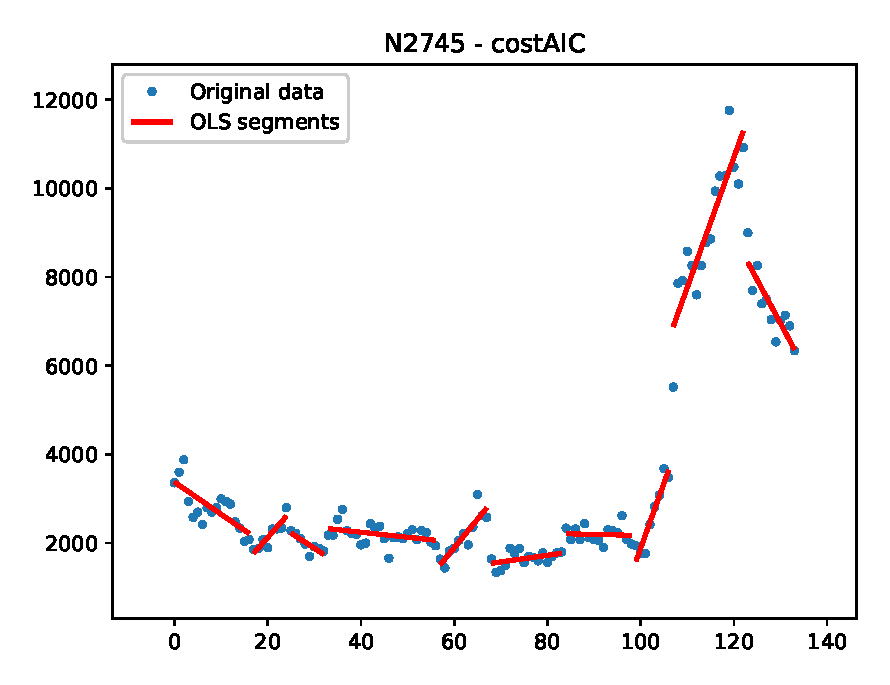
\includegraphics[width=0.495\textwidth]{N2745-costAIC}
		%\label{fig:AICcost}%
	}%
	\subfloat[\centering]{%
		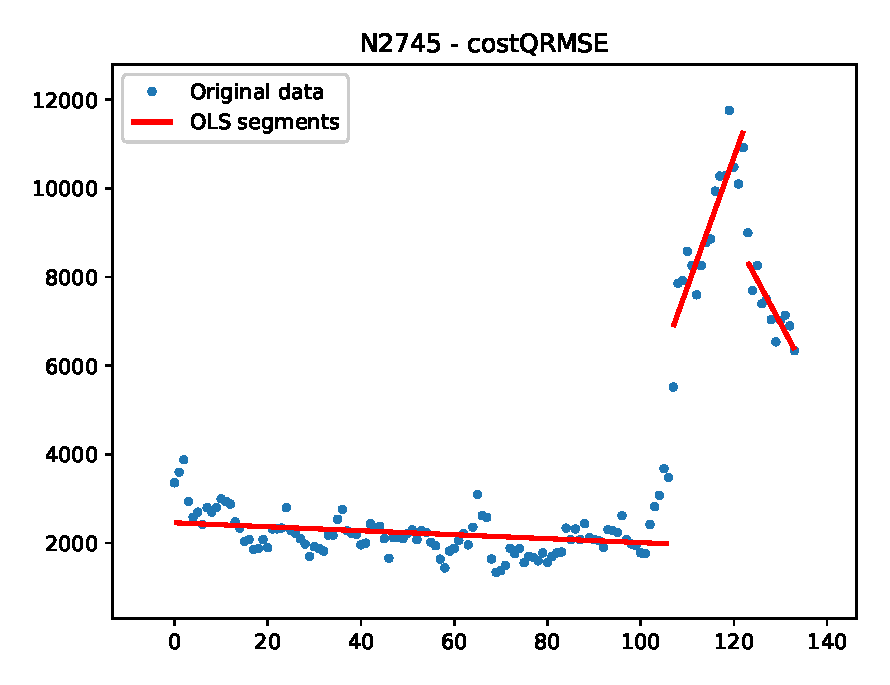
\includegraphics[width=0.495\linewidth]{N2745-costQRMSE}%
		%\label{fig:QRMSEcost}%
	}%
	\caption{Segmentations derived from different cost functions, M3 data series N2745, maximum 10~segments. (\textbf{a}) AIC cost segmentation. (\textbf{b}) QRMSE cost segmentation.}
	\label{fig:twocosts}
\end{figure}


When AIC is used as the cost function (Figure~\ref{fig:twocosts}a), the~resulting model exploits the full fragmentation allowed by the constraints, producing a segmentation with the maximum number of segments in order to achieve a close fit to the observed data points. In~contrast, when QRMSE is used (Figure~\ref{fig:twocosts}b), the~resulting segmentation tends to favor longer segments, tolerating a higher variance of observations around the fitted segments and thereby producing a smoother representation of the~series.

These results demonstrate the impact of the choice of cost function on the balance between fidelity to local fluctuations and the reduction of the number of~segments.



{We emphasize that there is no universally “correct” cost function for segmentation. Different criteria emphasize different characteristics of the fitted model and may therefore align better or worse with the expectations placed on the resulting segments. Beyond~these modeling preferences, the~statistical properties of the series itself also play an important role in determining which cost function performs more satisfactorily.
In light of these considerations, all subsequent analyses were conducted using AIC and QRMSE as the reference cost functions. AIC is retained because it is widely adopted in the changepoint detection literature, while QRMSE is selected because it represents a practical compromise between the tendency of MSE to over-fragment and that of RMSE to favor excessively long segments. It yields smoother segmentations that are often more aligned with visual expectations then either of the two more widely used alternatives. We emphasize that the selection of these two criteria is not driven by a formal statistical criterion, but~rather by the visual quality of the resulting segmentations and their complementary behavior across the benchmark instances.}
Figure~\ref{fig:categories} reports the optimal TSSP segmentation, obtained under the same constraints as in the previous experiment, for~four series belonging to different economic categories. The~results highlight the considerable heterogeneity present in these datasets. Even within a single category, series may exhibit markedly different structural properties, such as variability, seasonality, or~frequency of structural~changes.

\begin{figure}[H]
		\subfloat[\centering]{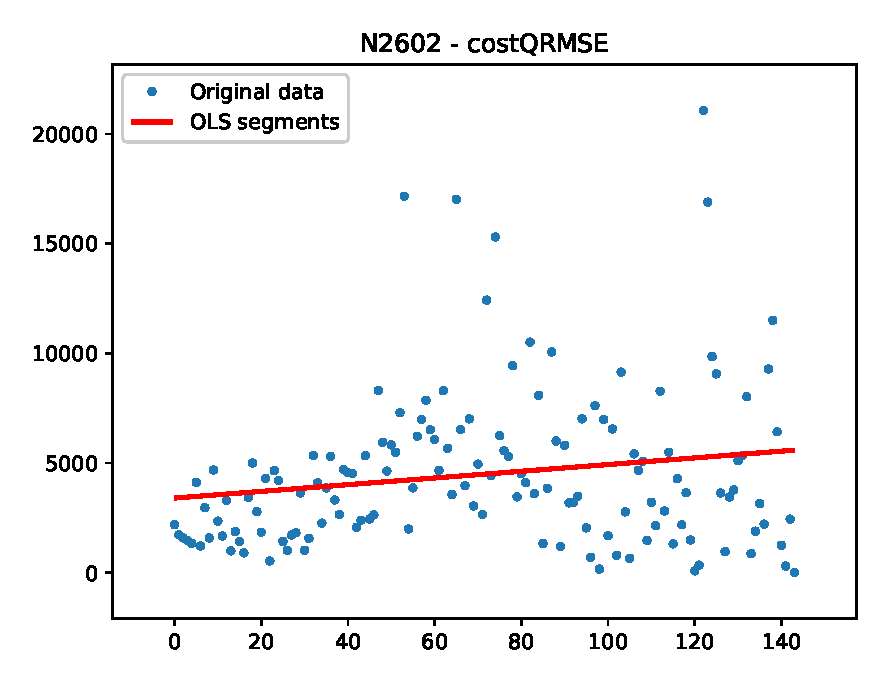
\includegraphics[width=0.495\textwidth]{N2602-costQRMSE.eps}}
		%\hfill
		\subfloat[\centering]{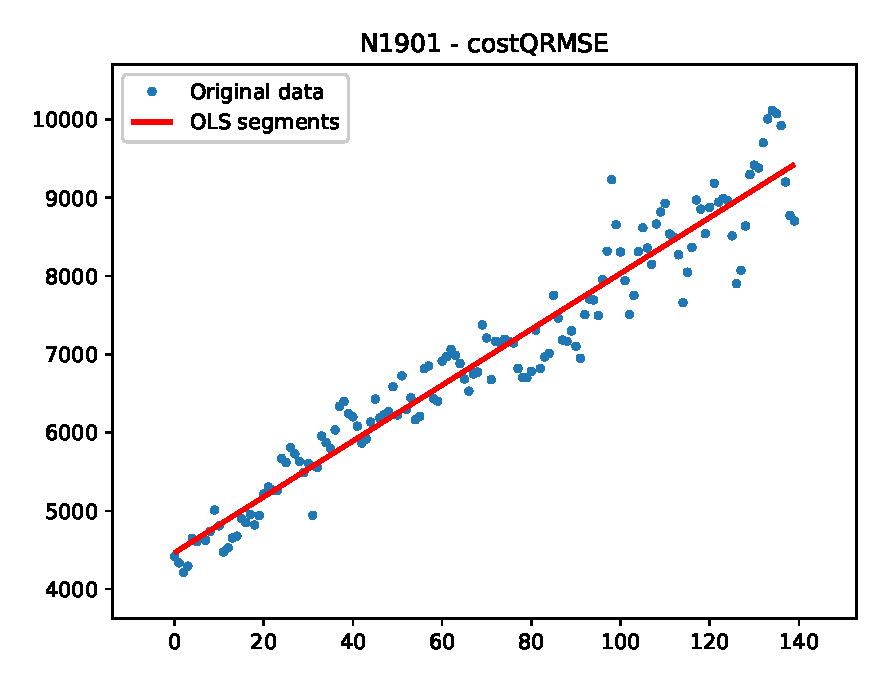
\includegraphics[width=0.495\textwidth]{N1901-costQRMSE.eps}}\\
		\subfloat[\centering]{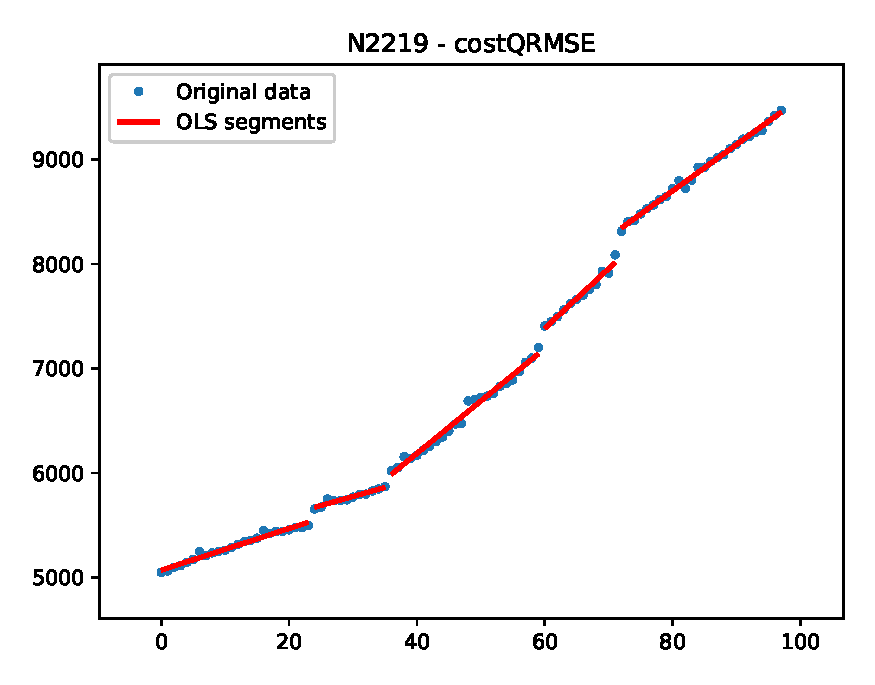
\includegraphics[width=0.495\textwidth]{N2219-costQRMSE.eps}}
		%\hfill
		\subfloat[\centering]{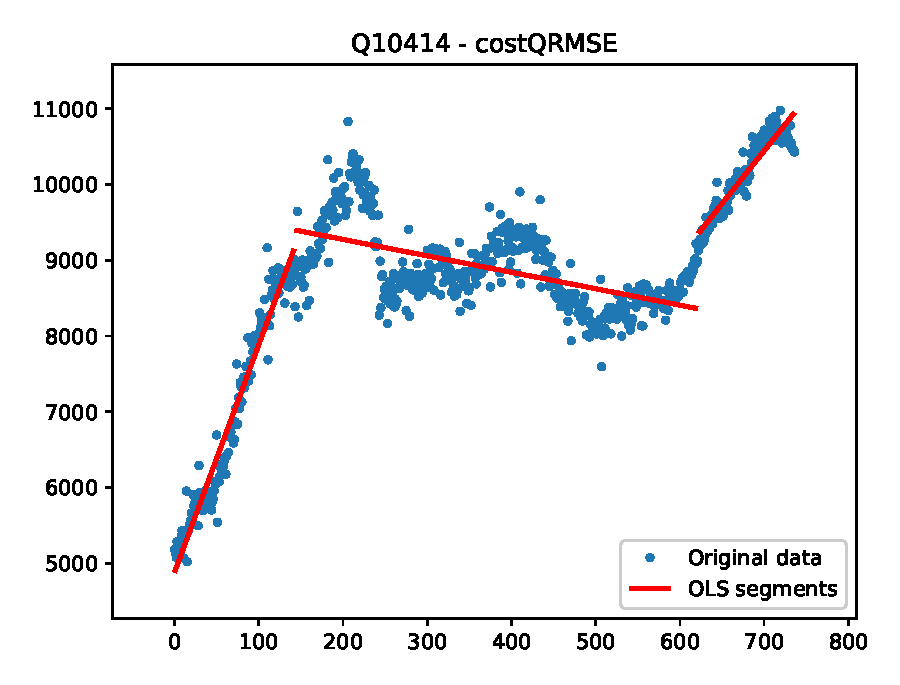
\includegraphics[width=0.495\textwidth]{Q10414-costQRMSE.eps}}
	\caption{ \textls[15]{Different data series categories: (\textbf{a}) Financial. (\textbf{b}) Industry. (\textbf{c}) Macroeconomics. \linebreak  (\textbf{d}) Microeconomics}.}
	\label{fig:categories}
\end{figure}

Because of this diversity, relying on a single cost function often entails a human-in-the-loop process in which the analyst repeatedly adjusts optimization control parameters to obtain satisfactory segmentations. In~contrast, selecting a cost function whose properties are known to match the statistical characteristics of the series can already guide the optimization toward the expected segmentation, reducing or eliminating the need for manual~intervention.

\subsubsection{Unconstrained~Segmentation}

In this section, we report the results obtained using the three unconstrained changepoint detection algorithms described earlier, namely PELT, Dynp, and Wild Binary Segmentation (WBS). 
The experiments were conducted on the M3, M4, and M6 benchmark datasets in order to provide baseline results for comparison with the proposed set-covering MILP framework. Both PELT and Dynp, which are exact optimization methods, were run using the implementation provided by the Ruptures library~\cite{rupweb}.

To ensure a consistent experimental setting across all algorithms, the~minimum segment length was fixed to eight observations. 
This choice prevents the detection of extremely short segments and aligns the unconstrained methods with the structural constraints that will later be~considered.

The parameters of the three algorithms were selected through preliminary calibration experiments carried out on a small number of representative series drawn from different dataset categories. For~each method, several parameter configurations were tested and the final parameter values were chosen so as to obtain segmentations whose number of segments is broadly comparable with the segmentation structures considered in the experiments with the proposed set-covering MILP~framework.

For the PELT algorithm, the~penalty parameters were set to $\beta=40$ for both the AIC function cost and the QRMSE function cost, with~\texttt{jump} $=1$ and \texttt{min\_size} $=8$.  

For Dynp, the~number of breakpoints was fixed to nine, corresponding to a target segmentation of ten segments. This choice was motivated by the fact that the experiments with the proposal framework consider segmentations with up to ten segments. The~minimum segment length was again set to eight observations. For~shorter series, the~requested number of breakpoints may not always be feasible under this constraint; in those cases, the~number of breakpoints was automatically reduced to the largest admissible~value.

For WBS, the~number of randomly generated intervals was fixed to $M=400$, while the minimum segment length was set to eight observations. The~threshold parameters were calibrated separately for the two cost functions and set to $\texttt{thr}_{\text{AIC}}=20$ and $\texttt{thr}_{\text{QRMSE}}=10$. 

The results reported in Tables~\ref{tab:PELTseriesAICQRMSE}--\ref{tab:WBSeriesAICQRMSE} highlight several differences among the three approaches. The~columns show the benchmark of the origin of the series, {\it Bench}; the~category of the set of series reported in the row, {\it Category}; and then separately for AIC and QRMSE, the median and maximum number of segments in the proposed solutions, {\it med.n}, {\it max.n}, and~the median and maximum CPU time for solving, {\it med.t}, {\it max.t}. In~Tables~\ref{tab:PELTseriesAICQRMSE} and \ref{tab:DYNPseriesAICQRMSE} we also added, for reference, the median and maximum CPU time used by MIP (inclusive of the setup time) for producing the solutions forcing the same number of segments as in Dynp, {\it med.t}, {\it max.t}. 
{No optimality gap is reported for these comparisons since TSSP, Pelt, and Dynp are all exact optimization methods that globally minimize the same additive objective and~are guaranteed to reach the same optimal cost. Therefore, reporting a cost gap would be uninformative; only computational times are compared.}
Since WBS is an heuristic method, in~Table~\ref{tab:WBSeriesAICQRMSE} we report the percentage cost gap between the solutions proposed by WBS and MIP, {\it med.gap} and {\it max.gap}.


\begin{table}[H]
	\caption{PELT: Data series results, AIC-QRMSE cost.}\label{tab:PELTseriesAICQRMSE}%
	
\begin{adjustwidth}{-\extralength}{0cm}
%\centering %% If there is a figure in wide page, please release command \centering, for Table, ``\textwidth" should be ``\fulllength"
	\begin{tabularx}\fulllength{CcCCCCCCCCCC}
		\toprule
		& & \multicolumn{4}{c}{\textbf{AIC}} & \multicolumn{4}{c}{\textbf{QRMSE}} & \multicolumn{2}{c}{\textbf{TSSP}} \\
		\textbf{Bench} & \textbf{Category} & \textbf{med.n} & \textbf{max.n} & \textbf{med.t} & \textbf{max.t}& \textbf{med.n} & \textbf{max.n} & \textbf{med.t} & \textbf{max.t} & \textbf{med.t} & \textbf{max.t}\\
		\midrule
		M3 & Demographic  & 3.0 & 7.0 & 0.0 & 0.0 & 3.0 & 4.0 & 0.0 & 0.0 & 0.41 & 0.59\\
		M3 & Finance      & 3.0 & 9.0 & 0.0 & 0.0 & 2.0 & 7.0 & 0.0 & 0.0 & 0.40 & 0.56\\
		M3 & Industry     & 1.0 & 2.0 & 0.0 & 0.0 & 1.0 & 12.0 & 0.0 & 0.0 & 0.55 & 0.69\\
		M3 & Macro        & 3.0 & 5.0 & 0.0 & 0.0 & 2.0 & 3.0 & 0.0 & 0.0 & 0.43 & 0.59\\
		M3 & Micro        & 1.0 & 2.0 & 0.0 & 0.0 & 1.0 & 1.0 & 0.0 & 0.0 & 0.33 & 0.5\\
		M3 & Other        & 3.0 & 4.0 & 0.0 & 0.0 & 1.0 & 4.0 & 0.0 & 0.0 & 0.27 & 0.45\\
		M4 & Demographic & 4.0 & 26.0 & 0.0 & 0.1 & 8.0 & 10.0 & 0.0 & 0.0 & 0.30 & 170.68\\
		M4 & Finance & 5.0 & 17.0 & 0.0 & 0.1 & 5.0 & 10.0 & 0.0 & 0.0 & 0.33 & 88.24 \\
		M4 & Industry & 5.0 & 10.0 & 0.0 & 0.1 & 6.0 & 7.0 & 0.0 & 0.0 & 0.58 & 71.77\\
		M4 & Macro & 5.0 & 35.0 & 0.0 & 0.1 & 2.0 & 17.0 & 0.0 & 0.0 & 0.41 & 153.33 \\
		M4 & Micro & 3.0 & 9.0 & 0.0 & 0.1 & 4.0 & 6.0 & 0.0 & 0.0 & 0.30 & 69.87\\
		M4 & Other & 7.0 & 28.0 & 0.0 & 0.0 & 2.0 & 9.0 & 0.0 & 0.0 & 1.03 & 55.1\\
		M6 & Finance & 6.5 & 8.0 & 0.0 & 0.0 & 1.0 & 1.0 & 0.0 & 0.0 & 2.72 & 3.10\\
		\bottomrule
	\end{tabularx}

\end{adjustwidth}

\end{table}

The first observation is that the number of segments detected varies substantially depending on the algorithm and cost function used.  The~AIC criterion generally favors more fragmented segmentations, whereas the QRMSE criterion tends to produce smoother segmentations with fewer change~points. 

\begin{table}[H]
	\caption{DYNP: Data series results, AIC-QRMSE cost.}\label{tab:DYNPseriesAICQRMSE}%
	\begin{adjustwidth}{-\extralength}{0cm}
%\centering %% If there is a figure in wide page, please release command \centering, for Table, ``\textwidth" should be ``\fulllength"
	\begin{tabularx}\fulllength{CcCCCCCCCCCC}
		\toprule
		& & \multicolumn{4}{c}{\textbf{AIC}} & \multicolumn{4}{c}{\textbf{QRMSE}} & \multicolumn{2}{c}{\textbf{TSSP}} \\
		\textbf{Bench} & \textbf{Category} & \textbf{med.n} & \textbf{max.n} & \textbf{med.t} & \textbf{max.t} & \textbf{med.n} & \textbf{max.n} & \textbf{med.t} & \textbf{max.t} & \textbf{med.t} & \textbf{max.t} \\
		\midrule
		M3 & Demographic  & 10.0 & 10.0 & 0.0 & 0.0 & 10.0 & 10.0 & 0.0 & 0.1 & 0.41 & 0.59\\
		M3 & Finance     & 10.0 & 10.0 & 0.0 & 0.1 & 10.0 & 10.0 & 0.0 & 0.0 & 0.40 & 0.56\\
		M3 & Industry     & 10.0 & 10.0 & 0.0 & 0.0 & 10.0 & 10.0 & 0.0 & 0.0 & 0.55 & 0.69\\
		M3 & Macro        & 10.0 & 10.0 & 0.0 & 0.1 & 10.0 & 10.0 & 0.0 & 0.0 & 0.43 & 0.59\\
		M3 & Micro        & 8.0 & 10.0 & 0.0 & 0.0 & 8.0 & 10.0 & 0.0 & 0.0 & 0.33 & 0.5\\
		M3 & Other        & 8.0 & 10.0 & 0.0 & 0.0 & 8.0 & 10.0 & 0.0 & 0.0  & 0.27 & 0.45\\
		M4 & Demographic & 10.0 & 10.0 & 0.0 & 2.5 & 10.0 & 10.0 & 0.0 & 2.8 & 0.30 & 170.68\\
		M4 & Finance & 10.0 & 10.0 & 0.0 & 2.5 & 10.0 & 10.0 & 0.0 & 2.7 & 0.33 & 88.24\\
		M4 & Industry & 10.0 & 10.0 & 0.0 & 2.5 & 10.0 & 10.0 & 0.0 & 2.7 & 0.58 & 71.77\\
		M4 & Macro & 10.0 & 10.0 & 0.0 & 3.7 & 10.0 & 10.0 & 0.0 & 4.1 & 0.41 & 153.33\\
		M4 & Micro & 10.0 & 10.0 & 0.0 & 2.5 & 10.0 & 10.0 & 0.0 & 2.7 & 0.30 & 69.87\\
		M4 & Other & 10.0 & 10.0 & 0.1 & 2.2 & 10.0 & 10.0 & 0.1 & 2.4 & 1.03 & 55.1\\
		M6 & Finance & 10.0 & 10.0 & 0.2 & 0.2 & 10.0 & 10.0 & 0.2 & 0.2& 2.72 & 3.10 \\
		\bottomrule
	\end{tabularx}
	\end{adjustwidth}
\end{table}
\vspace{-9pt}



\begin{table}[H]
	\caption{WBS: Data series results, AIC-QRMSE cost.}\label{tab:WBSeriesAICQRMSE}%
	\begin{adjustwidth}{-\extralength}{0cm}
%\centering %% If there is a figure in wide page, please release command \centering, for Table, ``\textwidth" should be ``\fulllength"
\begin{tabularx}\fulllength{CcCCCCCCCCcc}
	\toprule
	& & \multicolumn{4}{c}{\textbf{AIC}} & \multicolumn{4}{c}{\textbf{QRMSE}} & \multicolumn{2}{c}{\textbf{TSSP}} \\
	\textbf{Bench} & \textbf{Category} & \textbf{med.n} & \textbf{max.n} & \textbf{med.t} & \textbf{max.t} & \textbf{med.n} & \textbf{max.n} & \textbf{med.t} & \textbf{max.t} & \textbf{med.gap} & \textbf{max.gap} \\
	\midrule
	M3 & Demographic  & 10.0 & 11.0 & 0.3 & 0.3 & 5.0 & 8.0 & 0.2 & 0.3 & 1.30 &  9.26\\
	M3 & Finance      & 9.0 & 11.0 & 0.2 & 0.2 & 6.0 & 12.0 & 0.2 & 0.3 & 1.28 &  8.62\\
	M3 & Industry     & 5.0 & 12.0 & 0.2 & 0.5 & 2.0 & 14.0 & 0.1 & 0.4 & 0.89 & 64.41 \\
	M3 & Macro        & 8.0 & 11.0 & 0.2 & 0.3 & 5.0 & 6.0 & 0.2 & 0.3 & 0.25 &  3.84\\
	M3 & Micro        & 2.0 & 6.0 & 0.1 & 0.3 & 1.0 & 1.0 & 0.0 & 0.1& 0.47 &  1.83 \\
	M3 & Other        & 5.0 & 6.0 & 0.1 & 0.1 & 4.0 & 6.0 & 0.1 & 0.1 & 0.49 &  7.61\\
	M4 & Demographic & 9.0 & 55.0 & 0.2 & 2.9 & 11.0 & 37.0 & 0.2 & 2.6 & 5.57 & 29.54\\
	M4 & Finance & 10.0 & 56.0 & 0.2 & 2.7 & 9.0 & 39.0 & 0.2 & 2.3 & 7.15 & 60.91\\
	M4 & Industry & 10.0 & 27.0 & 0.3 & 2.7 & 8.0 & 11.0 & 0.3 & 2.0 & 3.31 & 26.15\\
	M4 & Macro & 9.0 & 69.0 & 0.2 & 3.3 & 7.0 & 50.0 & 0.2 & 3.2 & 3.30 & 44.30 \\
	M4 & Micro & 8.0 & 22.0 & 0.2 & 2.6 & 7.0 & 9.0 & 0.2 & 2.1 & 2.29 & 19.43\\
	M4 & Other & 10.0 & 51.0 & 0.4 & 2.5 & 8.0 & 31.0 & 0.3 & 2.2 & 3.58 & 29.82\\
	M6 & Finance & 17.0 & 21.0 & 0.7 & 0.8 & 1.0 & 3.0 & 0.2 & 0.4 & 0.00 & 33.05\\
	\bottomrule
\end{tabularx}
\end{adjustwidth}
\end{table}



The influence of this formulation is clearly evident in Table~\ref{tab:PELTseriesAICQRMSE}. When the PELT algorithm is used with the same penalty parameter, $\beta = 40$, for~both cost functions, the~QRMSE criterion generally produces fewer segments than the AIC criterion across most dataset categories. 
For instance, the~average number of detected segments decreases notably in several M4 categories under QRMSE, reflecting the criterion's reduced tendency to split long~segments.

Of the three methods, PELT often produces the fewest segments, reflecting the influence of the penalty term in the objective function. 
Dynp, on~the other hand, aims to generate segmentations closer to the desired number of ten segments, since the number of breakpoints is fixed. Finally, WBS typically exhibits the greatest variability in the number of detected segments due to the interval sampling~procedure. 

Of the two algorithms, PELT is usually the fastest, since its pruning strategy enables it to discard many candidate changepoints during the search process.
The Dynp algorithm generally takes slightly longer to run because it relies on a dynamic programming procedure whose complexity increases with the length of the series and the number of requested breakpoints. 
In contrast, WBS is not an exact optimization method; it repeatedly evaluates change-point statistics over a large number of randomly generated intervals ($M = 400$ in our experiments), which increases the computational burden. 
Consequently, despite its heuristic approach, WBS typically requires longer CPU times compared to the other two~methods.

We also ran the TSSP model while constraining it to generate exactly the same number of segments as Dynp, in~order to allow a fair performance comparison in a setting compatible with the other algorithms. In~this case, both TSSP and Dynp yield optimal solutions; therefore, only the computational times are reported for~TSSP.

The higher asymptotic complexity and longer setup time of TSSP are evident in Tables~\ref{tab:PELTseriesAICQRMSE} and \ref{tab:DYNPseriesAICQRMSE}. In~particular, the~degradation in TSSP performance becomes apparent for longer time~series.

Nevertheless, computational times remain below three minutes, even for instances leading to constraint matrices with nearly 1000 rows and more than 300,000 columns (see discussion on TSSP and TSSC later on). This demonstrates the practical viability of relying on state-of-the-art solvers, even for time series whose length would normally motivate data aggregation (e.g., subsampling or smoothing) for visualization~purposes.

Finally, Table~\ref{tab:WBSeriesAICQRMSE} compares the relative effectiveness of TSSP and WSB by reporting the percentage deviation of the cost of the solution produced by WSB from that of TSSP, computed on the same instance and for the same number of segments. The~median percentage error of WSB is generally small, with~values below 3\% and equal to 0\% for the M6 series. However, in~some cases, the heuristic fails to converge to solutions of acceptable~quality.

\subsubsection{Constrained~Segmentation}

In this section, we consider globally constrained series; therefore, the~only suitable models for application are the TSSP and its heuristic relaxation, the~TSSC. In~the examples, the~models were constrained to propose a maximum of ten segments (rather than an exact number of ten, as~managed by Dynp), as~well as a minimum segment length of eight. However, any of the additional constraints listed in Section~\ref{subsec:additional_constraints} could have been~included.

The results are summarized in Tables~\ref{tab:seriesQRMSE} and \ref{tab:seriesAIC}. The~columns show compatible data in both tables: the benchmark set of the origin of the series ({\it bench}), the~category of the series ({\it category}), the~average and maximum number of data points in the group series ({\it avg.n} and {\it max.n}), the~corresponding average and maximum number of generated runs ({\it avg.nrun} and {\it max.nrun}), the~average and maximum number of chosen segments ({\it avg.nseg} and {\it max.nsegm}), and~the average and maximum CPU time in seconds to solve the extended SCP model, inclusive of the time needed to generate the runs ({\it avg.t} and {\it max.t}).

\begin{table}[H]
\caption{Data series results, QRMSE cost.}\label{tab:seriesQRMSE}%
\begin{adjustwidth}{-\extralength}{0cm}
%\centering %% If there is a figure in wide page, please release command \centering, for Table, ``\textwidth" should be ``\fulllength"
\begin{tabularx}\fulllength{CcCCccCCCC}
\toprule
\textbf{Bench} & \textbf{Category} & \textbf{avg.n} & \textbf{max.n} & \textbf{avg.nrun} & \textbf{max.nrun} & \textbf{avg.nseg} & \textbf{max.nseg} & \textbf{avg.t} & \textbf{max.t} \\
\midrule
		M3 & Demographic & 122.6 & 138 &  7073.2 &   8646 & 3.8 &  7 &  0.6 & 1 \\
		M3 & Finance     & 124.8 & 144 &  7267.6 &   9453 & 3.6 &  9 &  0.1 & 0.1 \\
		M3 & Industry    & 139   & 144 &  8789.2 &   9453 & 1   &  1 &  0.1 & 0.1 \\
		M3 & Macro       & 128   & 144 &  7532.2 &   9453 & 2   &  5 &  0.1 & 0.1 \\
		M3 & Micro       & 91.8  & 126 &  4027.8 &   7140 & 1   &  1 &  0.1 & 0.1 \\
		M3 & Other       & 80.8  & 120 &  2952.2 &   6441 & 3.4 &  6 &  0.1 & 0.1 \\
		M4 & Demographic & 241.8 & 735 & 54,101.2 & 245,350 & 4   &  7 & 57.6 & 288 \\
		M4 & Finance     & 246   & 738 & 54,945.4 & 247,456 & 6.2 & 10 & 61.6 & 308 \\
		M4 & Industry    & 258.4 & 737 & 56,492   & 246,753 & 4.6 &  7 & 60   & 298 \\
		M4 & Macro   	 & 280   & 866 & 74,559.8 & 339,900 & 5.6 & 10 &106.6 & 532 \\
		M4 & Micro   	 & 232.8 & 737 & 53,371.2 & 246,753 & 2.8 &  7 & 58.4 & 292 \\
		M4 & Other   	 & 260.4 & 701 & 53,106.2 & 222,778 & 4.8 & 10 & 57.6 & 286 \\
		M6 & Finance 	 & 257.8 & 265 & 30,394.2 &  32,131 & 4.2 &  7 &  7.0 & 25 \\
\bottomrule
\end{tabularx}
\end{adjustwidth}
\end{table}



\begin{table}[H]
	\caption{Data series results, AIC cost.}\label{tab:seriesAIC}%
	\begin{adjustwidth}{-\extralength}{0cm}
%\centering %% If there is a figure in wide page, please release command \centering, for Table, ``\textwidth" should be ``\fulllength"
\begin{tabularx}\fulllength{CcCCccCCCC}
	\toprule
		\textbf{Bench} & \textbf{Category} & \textbf{avg.n} & \textbf{max.n} & \textbf{avg.nrun} & \textbf{max.nrun} & \textbf{avg.nseg} & \textbf{max.nseg} & \textbf{avg.t} & \textbf{max.t} \\
		\midrule
		M3 & Demographic & 122.6 & 138 & 7073.2 & 8646 & 9.4 & 10 & 0.2 & 1 \\
		M3 & Finance     & 124.8 & 144 & 7267.6 & 9453 & 9.6 & 10 & 0.1 & 0.1 \\
		M3 & Industry    & 139 	 & 144 & 8789.2 & 9453 & 10 & 10  & 0.1 & 0.1 \\
		M3 & Macro       & 128   & 144 & 7532.2 & 9453 & 10 & 10  & 0.1 & 0.1 \\
		M3 & Micro       & 91.8  & 126 & 4027.8 & 7140 & 6.6 & 10 & 0.1 & 0.1 \\
		M3 & Other       & 80.8  & 120 & 2952.2 & 6441 & 7.4 & 9  & 0.1 & 0.1 \\
		M4 & Demographic & 241.8 & 735 & 54,101.2 & 245,350 & 10  & 10 & 58.4 & 292 \\
		M4 & Finance 	 & 246   & 738 & 54,945.4 & 247,456 & 10  & 10 & 65.2 & 325 \\
		M4 & Industry 	 & 258.4 & 737 & 56,492   & 246,753 & 8.8 & 10 & 62.4 & 310 \\
		M4 & Macro 		 & 280   & 866 & 74,559.8 & 339,900 & 10  & 10 & 105.8 & 528 \\
		M4 & Micro 		 & 232.8 & 737 & 53,371.2 & 246,753 & 10  & 10 & 60.4 & 302 \\
		M4 & Other 		 & 260.4 & 701 & 53,106.2 & 222,778 & 10  & 10 & 57.8 & 285 \\
		M6 & Finance 	 & 257.8 & 265 & 30,394.2 & 32131 & 10.0 & 10 & 5.9 & 7 \\
		\bottomrule
	\end{tabularx}
	\end{adjustwidth}
\end{table}


Table~\ref{tab:seriesQRMSE} reports the aggregate results obtained with the TSSP model using QRMSE as the cost function. The~results show that relatively short series—up to a few hundred observations—lead to integer programming instances of moderate size that can be solved very efficiently even on standard~hardware.

As the length of the series increases, the~non-polynomial complexity of the exact integer programming search becomes more apparent. When the series approaches about 500 observations, solution times begin to require minutes of CPU time. This increase is primarily due to the rapid growth of the IP formulation, whose constraint matrix (the “tableau”) may reach dimensions close to 1000 rows and more than 300,000~columns.


Table~\ref{tab:seriesAIC} reports the results obtained on the same set of series when AIC is used as the cost function. Since the cost function affects only the data preparation phase—namely the computation of the costs associated with the feasible segments—the size of the resulting IP instances remains unchanged, and~the dimensions of the constraint matrices are therefore identical to those reported in Table~\ref{tab:seriesQRMSE}.

The CPU time required for the optimization, however, is influenced by the numerical values of the costs, although~this effect is relatively limited. The~most notable difference between Tables~\ref{tab:seriesQRMSE} and \ref{tab:seriesAIC} concerns the number of segments in the optimal solutions. When AIC is used, the~optimal segmentation frequently saturates the imposed upper bound on the number of segments, whereas QRMSE tends to produce solutions with a consistently smaller number of~segments.


A final remark concerns the relative effectiveness of the two models, TSSP and TSSC. This comparison is reported in Table~\ref{tab:SPP_SCP}. The~columns show the following: the instance name {\it name}, the~number of rows {\it rows} and columns {\it cols} of the constraint matrix, and~the number of nonzero coefficients {\it nonzeros}. The~remaining columns report the CPU time, in~seconds, required to generate all feasible segment runs {\it truns}, to~solve the instance using model TSSP {\it tSSP}, and~to solve it using model TSSC {\it tSSC}. The~latter includes the time required by the fixing heuristic used to ensure feasibility of the final TSSC solution. Column {\it GAP} reports the percentage cost gap between the heuristic TSSC solution and the optimal TSSP~solution.

The table summarizes results for the longest series included in our benchmark set. The~figures highlight the limited computational burden associated with the preliminary generation of segment runs, as~well as the effectiveness of modern MIP solvers, which are able to handle matrices of substantial size and densities exceeding 36\% within a few minutes of CPU time. As~expected, the~{\it TSSP} model requires longer solution times, whereas {\it TSSC} is, on average, about 40\% faster. The~fixing heuristic runs in negligible time and produces solutions whose average optimality gap with respect to {\it TSSP} remains consistently below~1\%.


\begin{table}[H]
	\caption{Partitioning vs. covering comparison.}\label{tab:SPP_SCP}%
	\begin{tabularx}\textwidth{CCccCCCC}
		\toprule
		\textbf{Name} & \textbf{Rows} & \textbf{Cols} & \textbf{Nonzeros} & \textbf{Truns} & \textbf{GAP} & \textbf{tSSP} & \textbf{tSSC} \\
		\midrule
Q13050 & 736 & 245,350 &  66,244,500 & 2 & 0.06 & 219 & 162 \\
Q22221 & 739 & 247,456 &  67,060,576 & 4 & 0.81 & 294 & 119 \\
Q15697 & 738 & 246,753 &  66,787,812 & 4 & 0.16 & 275 & 201 \\
Q5109  & 867 & 339,900 & 108,201,500 & 6 & 0.60 & 467 & 211 \\
Q10414 & 738 & 246,753 &  66,787,812 & 3 & 0.33 & 326 & 197 \\
Q23661 & 702 & 222,778 &  57,476,724 & 6 & 0.99 & 242 & 143 \\
		\bottomrule
	\end{tabularx}
\end{table}





%\begin{figure*}[ht]
%    \centering
%    \subfloat[Bitcoin - USD exchange rate]{%
%        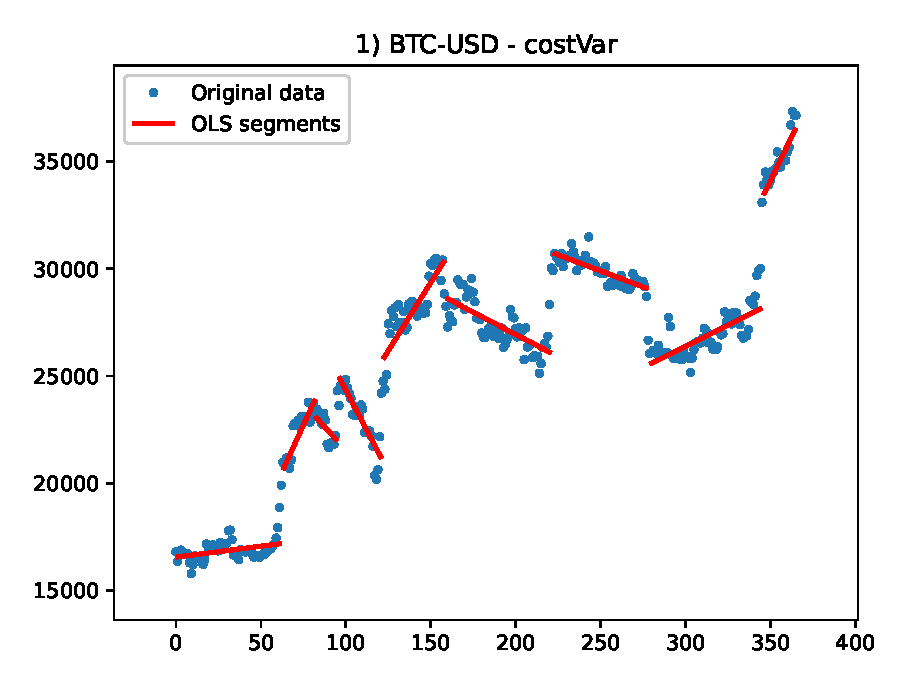
\includegraphics[width=0.45\textwidth]{BTC-USDcostVar.eps}
%        \label{fig:bitcoins}%
%        }%
%    \hfill%
%    \subfloat[Covid Italy 2022]{%
%        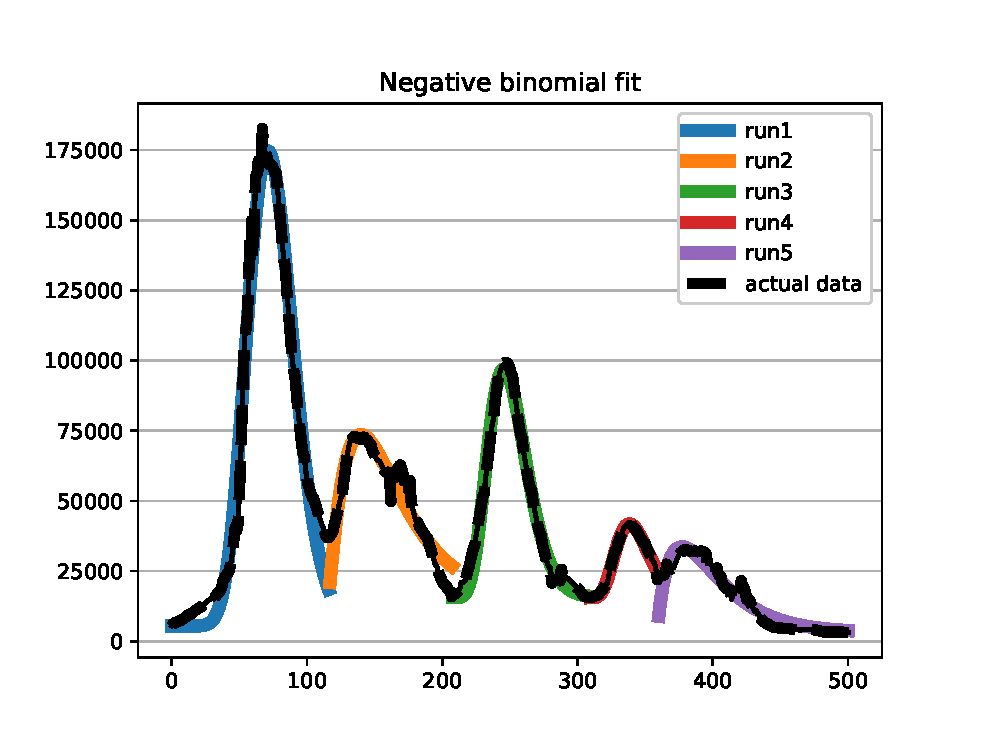
\includegraphics[width=0.45\linewidth]{negativeBinFit.eps}%
%        \label{fig:health}%
%        }%
%    \caption{Economics and healthcare dataseries}
%    \label{fig:nonenv}
%\end{figure*}


	\subsubsection{Cutting Planes~Insertions}
	
	When dealing with global constraints—i.e., constraints acting on the entire series rather than on individual segments—the number of constraints to be included in the formulation may become prohibitive. To~address this limitation, such constraints can be incorporated in a cutting-plane fashion, being added only when they are violated and thus effectively restricting the feasible~region.
	
	As an illustrative example, consider a setting in which the desired segmentation must satisfy three types of global constraints: a {\it minimum cardinality}, a~{\it maximum cardinality}, and~{\it change direction} constraints. While the first two can be enforced by a single inequality each, the~third class induces a number of constraints that grows quadratically with the length of the time series. The~corresponding formulation is denoted as $TSSP_G$
	\begin{alignat}{4}
		(TSSP_G) \hspace{0.5cm} z_{TSSC} = \min     &\; \sum_{j=1}^{nruns} c_j x_{j}  \label{eq:SCPobjG} \\
		s.t. &\; \sum_{j=1}^{nruns}a_{ij}x_{j} = 1, & \hspace{1.5cm} i=1,\dots,npoints  \label{eq:SCPcovG} \\
		&\; \sum_{j=1}^{nruns} x_{j} \leq maxruns \label{eq:SPPmaxG}\\
		&\; \sum_{j=1}^{nruns} x_{j} \geq minruns \label{eq:SPPminG}\\
		&\; x_j + \sum_{i \in I_j} x_i \leq 1  & \hspace{1.5cm} j=1,\dots,nruns  \label{eq:updown}\\
		&\; x_j \in \{0,1\},                   &\; j=1,\dots,nruns  \label{eq:SCPvarG}
	\end{alignat}
	\noindent where the notation $I_j$ in constraint (\ref{eq:updown}) denotes the index set of variables associated with segments having the same slope as the segment associated with variable $x_j$.
	
	We implemented this formulation by adding constraints (\ref{eq:updown}) in a cutting-plane fashion. In~our setting, the~separation routine is straightforward: for each selected variable, it suffices to check whether another contiguous segment with the same slope is simultaneously included in the solution. If~this occurs, a~cut is generated, forbidding the corresponding variables from being selected together. The~cut is then lifted to include all contiguous segments sharing the same slope as the one under~consideration.
	
	Change direction constraints are of particular interest when modeling periodic series. To~evaluate their impact, we selected the ten series from the M3 benchmark set exhibiting the highest degree of seasonality and instantiated formulation $TSSP_G$ with $minruns = 5$ and $maxruns = 25$. The~results are reported in Table~\ref{tab:global}, where, for~both AIC and QRMSE cost functions, we provide the number of segments in the final solution ($n.segm$), the~CPU time required to obtain the solution ($t.cpu$), and~the number of cuts generated during the optimization ($n.cuts$).
	
	\begin{table}[H]
		\caption{Global constraints.}\label{tab:global}%
		
\begin{adjustwidth}{-\extralength}{0cm}
%\centering %% If there is a figure in wide page, please release command \centering, for Table, ``\textwidth" should be ``\fulllength"
		\begin{tabularx}\fulllength{CCcCCCCCC}
			\toprule
			& & &  \multicolumn{3}{c}{\textbf{AIC}} & \multicolumn{3}{c}{\textbf{QRMSE}}\\
			\textbf{Series} & \textbf{N} & \textbf{Category} & \textbf{n.segm} & \textbf{t.cpu} & \textbf{n.cuts} & \textbf{n.segm} & \textbf{t.cpu} & \textbf{n.cuts} \\
			\midrule
			N1906 & 134 &    INDUSTRY & 22 &    8.81 &   5 & 5 &   7.97 & 4 \\
			N2577 & 134 &     FINANCE &  9 & 5577.86 & 921 & 5 & 150.94 & 178 \\
			N2465 & 132 &       MACRO & 22 &  859.49 & 299 & 5 & 259.80 & 37 \\
			N2747 & 132 & DEMOGRAPHIC & 22 &    1.63 &   0 & 5 &   5.71 & 2 \\
			N2504 & 108 &       MACRO & 17 &  354.38 & 262 & 5 &  47.67 & 44 \\
			N2572 & 134 &     FINANCE &  5 &   17.05 &   6 & 5 &  21.48 & 9 \\
			N2568 & 134 &     FINANCE &  5 &   13.20 &   6 & 5 &  21.16 & 9 \\
			N2799 &  96 &       OTHER & 16 &    0.29 &   0 & 5 &   6.91 & 18 \\
			N1907 & 144 &    INDUSTRY & 24 &    8.37 &   4 & 5 &   5.22 & 3 \\
			N2798 &  96 &       OTHER & 16 &    0.30 &   0 & 5 &   1.00 & 1 \\
			\bottomrule
		\end{tabularx}

\end{adjustwidth}
		%\end{adjustwidth}
	\end{table}
	
	Several observations can be drawn from the results reported in Table~\ref{tab:global}. First, highly seasonal series arise across a wide range of domains; indeed, even within the first ten selected series, most of the categories represented in the M3 benchmark are covered. Second, the~QRMSE cost function tends to model the series using a small number of long segments. Since all selected instances exhibit relatively high-frequency seasonality, this results in segmentations with the minimum number of segments allowed for by the constraints. In~contrast, AIC tends to favor more fragmented segmentations, adhering more closely to the observed data points within the limits imposed by the~constraints.
	
	The number of cuts required varies significantly across instances, although~it remains substantially smaller than the total number of potential cuts. This variability has a marked impact on the computational effort: while most instances are solved quickly, a~small subset requires a substantially larger number of cuts, leading to a sharp increase in CPU~time.
	
 Figure~\ref{fig:changedir} illustrates the impact of the change direction constraints. Figure~\ref{fig:changedir}a presents the optimal solution obtained with the AIC cost for series N2747 without imposing these constraints, while Figure~\ref{fig:changedir}b shows the corresponding solution when the constraints are enforced. The~difference between the two highlights the additional search effort required to transform the former solution into the~latter.
	\vspace{-11pt}
	
	\begin{figure}[H]
		\subfloat[\centering]{%
			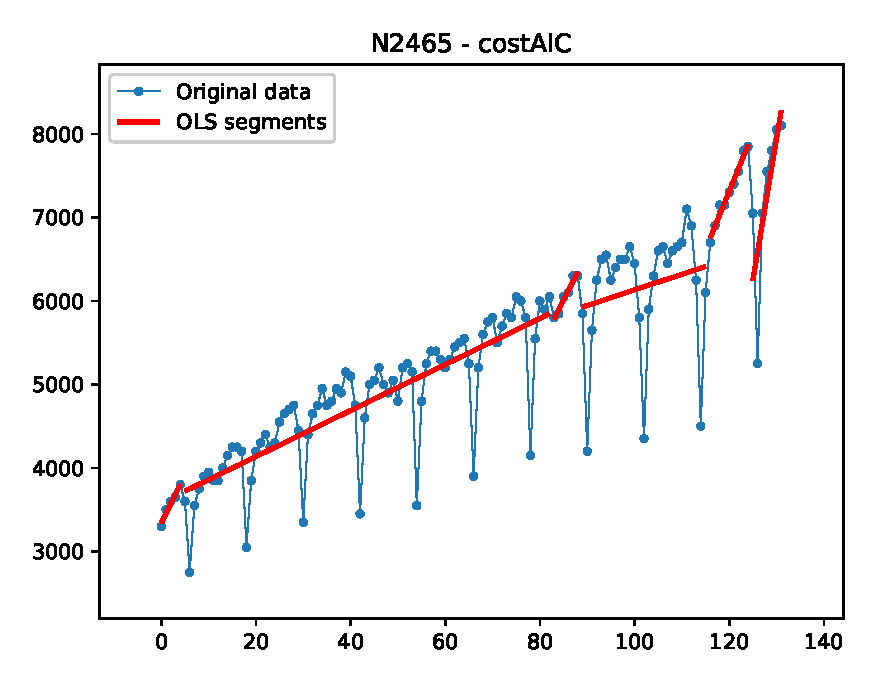
\includegraphics[width=0.49\textwidth]{figs/N2465-bare-costAIC.eps}
			%\label{fig:bareAIC}%
		}%
		\hfill%
		\subfloat[\centering]{%
			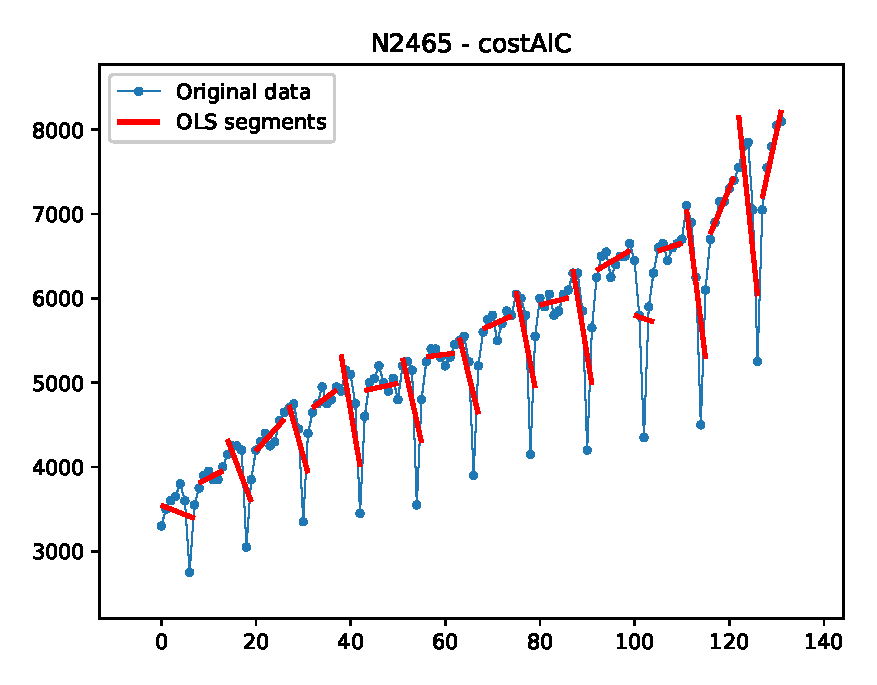
\includegraphics[width=0.49\linewidth]{figs/N2465-ud-costAIC.eps}%
			%\label{fig:cdAIC}%
		}%
		\caption{Series N2465, impact of change direction~constraints. (\textbf{a}) Without change direction constraints. (\textbf{b}) With change direction constraints}. \label{fig:changedir}
	\end{figure}
	
	
	Finally, Figure~\ref{fig:sameSegm} illustrates the impact of the remaining constraints. The~AIC cost function is prone to fragmentation, and is therefore primarily affected by the constraint on the maximum number of segments. In~contrast, QRMSE favors longer segments and is thus more sensitive to the constraint on the minimum number of~segments.
	

\vspace{-11pt}
\begin{figure}[H]
	\subfloat[\centering]{%
		
\includegraphics[width=0.49\textwidth]{figs/N2465-costAIC}
		%\label{fig:wAIC}%
	}%
	\hfill%
	\subfloat[\centering]{%
		
\includegraphics[width=0.49\linewidth]{figs/N2465-costQRMSE}%
		%\label{fig:wQRMSE}%
	}%
	\caption{Series N2465, equivalent~constraints. (\textbf{a}) AIC cost function. (\textbf{b}) QRMSE cost function}.
	\label{fig:sameSegm}
\end{figure}

	When the number of segments is fixed to be the same, Figure~\ref{fig:sameSegm}a shows that AIC tends to adhere more closely to the high-slope runs on the right-hand side of the series, whereas QRMSE favors longer segments spanning those~regions.
	
	

\subsubsection{Nonlinear~Models}

We emphasize that the validity of the proposed framework is not restricted to piecewise linear regression: any parametric or nonparametric trend function can be adopted for computing the segment-specific error cost. Figure~\ref{fig:covid} illustrates the segmentation obtained by applying the model to the time series of total infected patients in Italy during the first year and a half (500 data points) of the COVID-19 pandemic. The~epidemic evolved through successive waves, each of which can be effectively approximated by a trend following a negative binomial pattern. Accordingly, the~formulation of Section~\ref{sec:SCPmodel} is applied by computing, for~each feasible run, the~fitting error associated with a negative binomial model. The~subsequent optimization procedure remains~unchanged.


\vspace{-3pt}
\begin{figure}[H]
	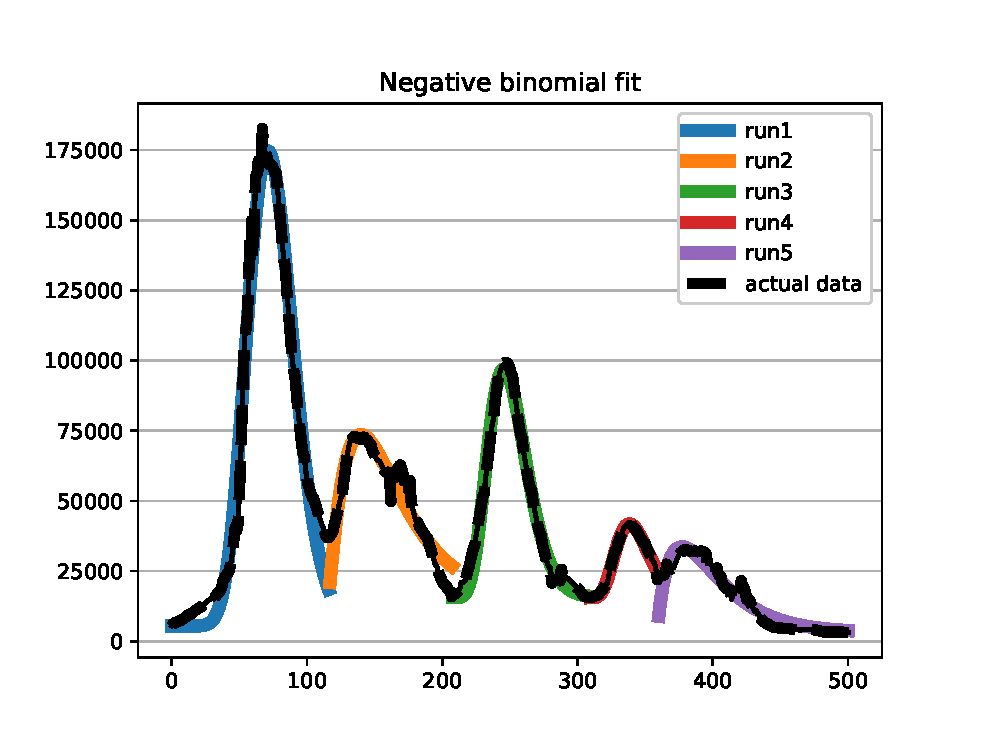
\includegraphics[width=0.78\linewidth]{negativeBinFit.eps}%
	\caption{COVID diffusion in~Italy.}
   \label{fig:covid}%
\end{figure}

As a final remark, the~changepoints identified on this COVID-19 series admit a clear epidemiological interpretation, as~they correspond to phases in which a new wave of contagion emerged or was reasonably expected to~emerge.


%% Example of a page in landscape format (with table and table footnote).
%\startlandscape
%\begin{table}[H] %% Table in wide page
%%\isPreprints{\centering}{} % This command is only used for ``preprints''.
%\caption{This is a very wide table.\label{tab3}}
%	\begin{tabularx}{\textwidth}{CCCC}
	%		\toprule
	%		\textbf{Title 1}	& \textbf{Title 2}	& \textbf{Title 3}	& \textbf{Title 4}\\
	%		\midrule
	%		Entry 1		& Data			& Data			& This cell has some longer content that runs over two lines.\\
	%		Entry 2		& Data			& Data			& Data\textsuperscript{1}\\
	%		\bottomrule
	%	\end{tabularx}
%%\isPreprints{}{% This command is only used for ``preprints''.
	%	\begin{adjustwidth}{+\extralength}{0cm}
		%%} % If the paper is ``preprints'', please uncomment this parenthesis.
	%		\noindent\footnotesize{\textsuperscript{1} This is a table footnote.}
	%%\isPreprints{}{% This command is only used for ``preprints''.
		%	\end{adjustwidth}
	%%} % If the paper is ``preprints'', please uncomment this parenthesis.
%\end{table}
%\finishlandscape


\section{Conclusions}              			\label{sec:conclusions}

In this work, we proposed a novel formulation of the changepoint detection (CPD) problem based on an extended set partitioning (SPP) model, together with a relaxed set covering (SCP) variant. The~proposed approach provides an exact optimization framework that remains computationally competitive with state-of-the-art dynamic programming methods on instances of moderate size and can be used in settings where such methods are applicable.
We remark that that the SCP variant, while computationally more efficient than the SPP formulation, yields a heuristic solution to the CPD problem: the postprocessing step required to resolve overlapping runs does not preserve the global optimality guarantee. However, in~our experiments, the~average optimality gap remained consistently below $1\%$, confirming the practical effectiveness of the~heuristic.
	
A key advantage of the ILP formulation lies in its modeling flexibility. By~representing feasible segments as atomic decision variables, the~framework can naturally accommodate a wide range of structural and global constraints that are difficult or impractical to incorporate within classical dynamic programming approaches. This allows for the method to address a broader class of CPD problems, extending its applicability beyond traditional settings.

\textls[-15]{Computational results on a diverse collection of benchmark time series, including those from the M3, M4, and~M6 competitions, demonstrate the practical viability of the approach. The~experiments show that the method is capable of producing high-quality segmentations across heterogeneous datasets while maintaining reasonable computational~effort.}

Several directions for future research emerge from this work. A~natural extension is the development of formulations that jointly optimize both the segmentation and the parameters of the segment models, rather than relying on a preprocessing phase to enumerate feasible segments. Further improvements may be obtained by integrating advanced decomposition techniques, such as column generation or branch-and-price methods, to~handle larger instances more efficiently. Finally, the~design of specialized cutting planes and problem-specific heuristics could further enhance scalability and solution~quality.

%%%%%%%%%%%%%%%%%%%%%%%%%%%%%%%%%%%%%%%%%%
\vspace{6pt}


%%%%%%%%%%%%%%%%%%%%%%%%%%%%%%%%%%%%%%%%%%
\authorcontributions{ Conceptualization, V.M. and L.V.; Methodology, V.M. and L.V.; Software, V.M. and L.V.; Validation, V.M. and L.V.; Formal analysis, V.M. and L.V.; Investigation, V.M. and L.V.; Resources, V.M. and L.V.; Data curation, V.M. and L.V.; Writing---original draft, V.M. and L.V.; Writing---review and editing, V.M. and L.V.; Visualization, V.M. and L.V.; Supervision, V.M. and L.V.; Project administration, V.M. and L.V. All authors have read and agreed to the published version of the~manuscript.}

\funding{This research received no external funding.}

\informedconsent{Not applicable.}

\dataavailability{The data presented in this study are available in [the International Institute of Forecasters] at [\url{https://forecasters.org/resources/time-series-data/}  (accessed on 16 April 2016 %MDPI: Please provide the date you accessed the URL in the following format: “URL (accessed on Day Month Year)”.
)].}

\acknowledgments{During the preparation of this manuscript/study, the~authors used GenAI, Sonnet v.4.6, only for the purposes of syntax and style checking.}

\conflictsofinterest{The authors declare no conflicts of interest.}

\clearpage
%%%%%%%%%%%%%%%%%%%%%%%%%%%%%%%%%%%%%%%%%%
%% Optional

%% Only for journal Encyclopedia
%\entrylink{The Link to this entry published on the encyclopedia platform.}

\abbreviations{Abbreviations}{
The following abbreviations are used in this manuscript:\\

\noindent
\begin{tabular}{@{}ll}
IP   & Integer Programming\\
MIP  & Mixed Integer Programming\\
MILP & Mixed Integer Linear Programming\\
NP   & Nondeterministic Polynomial
\end{tabular}
}

%%%%%%%%%%%%%%%%%%%%%%%%%%%%%%%%%%%%%%%%%%
\isPreprints{}{% This command is only used for ``preprints''.
\begin{adjustwidth}{-\extralength}{0cm}
} % If the paper is ``preprints'', please uncomment this~parenthesis.

\reftitle{References}
% References, variant A: external bibliography
%\bibliography{mathematicsMain.bib}
\begin{thebibliography}{999}

\bibitem[Lovri{\'c} et~al.(2014)Lovri{\'c}, Milanovi{\'c}, and
  Stamenkovi{\'c}]{LMS14}
Lovri{\'c}, M.; Milanovi{\'c}, M.; Stamenkovi{\'c}, M.
\newblock Algorithmic Methods for Segmentation of Time Series: An Overview.
\newblock {\em J. Contemp. Econ. Bus. Issues} {\bf
  2014}, {\em 1},~31--53.

\bibitem[Aminikhanghahi and Cook(2017)]{AC17}
Aminikhanghahi, S.; Cook, D.J.
\newblock A Survey of Methods for Time Series Change Point Detection.
\newblock {\em Knowl. Inf. Syst.} {\bf 2017}, {\em
  51},~339--367.
\newblock {\url{https://doi.org/10.1007/s10115-016-0987-z}}.

\bibitem[Truong et~al.(2020)Truong, Oudre, and Vayatis]{TOV20}
Truong, C.; Oudre, L.; Vayatis, N.
\newblock Selective Review of Offline Change Point Detection Methods.
\newblock {\em Signal Process.} {\bf 2020}, {\em 167},~107299.
\newblock {\url{https://doi.org/10.1016/j.sigpro.2019.107299}}.

\bibitem[Keogh et~al.(2002)Keogh, Chu, Hart, and Pazzani]{KCHP02}
Keogh, E.; Chu, S.; Hart, D.; Pazzani, M.
\newblock An online algorithm for segmenting time series.  In \textit{Proceedings 2001 IEEE International Conference on Data Mining}; IEEE: Piscataway, NJ, USA %MDPI: We added the name of the title, publisher and their location. Please confirm. The following highlights are the same.
, 2001; pp. 289--296.


\bibitem[Auger and Lawrence(1989)]{AL89}
Auger, I.E.; Lawrence, C.E.
\newblock Algorithms for the optimal identification of segment neighborhoods.
\newblock {\em Bull. Math. Biol.} {\bf 1989}, {\em 51},~39--54.

\bibitem[Jackson et~al.(2005)Jackson, Scargle, Barnes, Arabhi, Alt, Gioumousis,
  Gwin, Sangtrakulcharoen, Tan, and Tsai]{JSB05}
Jackson, B.; Scargle, J.D.; Barnes, D.; Arabhi, S.; Alt, A.; Gioumousis, P.;
  Gwin, E.; Sangtrakulcharoen, P.; Tan, L.; Tsai, T.T.
\newblock An algorithm for optimal partitioning of data on an interval.
\newblock {\em IEEE Signal Process. Lett.} {\bf 2005}, {\em 12},~105--108.

\bibitem[Killick et~al.(2012)Killick, Fearnhead, and Eckley]{KFE12}
Killick, R.; Fearnhead, P.; Eckley, I.A.
\newblock Optimal detection of changepoints with a linear computational cost.
\newblock {\em J. Am. Stat. Assoc.} {\bf 2012},
  {\em 107},~1590--1598.

\bibitem[Rigaill(2010)]{R10}
Rigaill, G.
\newblock Pruned dynamic programming for optimal multiple change-point
  detection.
\newblock {\em arXiv} {\bf 2010}, arXiv:1004.0887.

\bibitem[Johnson(2013)]{J13}
Johnson, N.A.
\newblock A dynamic programming algorithm for the fused lasso and
  L0-segmentation.
\newblock {\em J. Comput. Graph. Stat.} {\bf 2013},
  {\em 22},~246--260.

\bibitem[Hocking et~al.(2013)Hocking, Rigaill, Fearnhead, and Bourque]{HRFB13}
Hocking, T.D.; Rigaill, G.; Fearnhead, P.; Bourque, G.
\newblock Learning sparse penalties for change-point detection using max-margin
  interval regression.  In \textit{International Conference on Machine Learning (ICML)}; PMLR: New York, NY, USA, 2013.

\bibitem[Bellman(1961)]{B61}
Bellman, R.
\newblock On the approximation of curves by line segments using dynamic
  programming.
\newblock {\em Commun. ACM} {\bf 1961}, {\em 4},~284.

\bibitem[Picard and Cook(1975)]{PC75}
Picard, D.; Cook, R.D.
\newblock Cross-validation of regression models.
\newblock {\em J. Am. Stat. Assoc.} {\bf 1975},
  {\em 79},~575--583.

\bibitem[Hudson(1966)]{H66}
Hudson, D.J.
\newblock Fitting segmented curves whose join points have to be estimated.
\newblock {\em J. Am. Stat. Assoc.} {\bf 1966},
  {\em 61},~1097--1129.

\bibitem[Fisher(1958)]{F58}
Fisher, W.D.
\newblock On grouping for maximum homogeneity.
\newblock {\em J. Am. Stat. Assoc.} {\bf 1958},
  {\em 53},~789--798.

\bibitem[Bertsimas et~al.(2016)Bertsimas, King, and Mazumder]{BKM16}
Bertsimas, D.; King, A.; Mazumder, R.
\newblock Best subset selection via a modern optimization lens.
\newblock {\em Ann. Stat.} {\bf 2016}, {\em 44},~813--852.

\bibitem[Prokhorov et~al.(2025)Prokhorov, Radchenko, Semenov, and
  Skrobotov]{PRSS25}
Prokhorov, A.; Radchenko, P.; Semenov, A.; Skrobotov, A.
\newblock Change-Point Detection in Time Series Using Mixed Integer Programming. \textit{arXiv}
  {\bf 2025}, \url{https://doi.org/10.48550/arXiv.2408.05665}.


\bibitem[Balinski(1969)]{B69}
Balinski, M.L.
\newblock {\em Integer Programming: Methods, Uses, Computation}; Academic
  Press:  Cambridge, MA, USA,
  1969.

\bibitem[Schrijver(2003)]{S03}
Schrijver, A.
\newblock {\em Combinatorial Optimization: Polyhedra and Efficiency}; Springer: Berlin/Heidelberg, Germany,
2003.

\bibitem[Box et~al.(2015)Box, Jenkins, Reinsel, and Ljung]{box2015}
Box, G.E.P.; Jenkins, G.M.; Reinsel, G.C.; Ljung, G.M.
\newblock {\em Time Series Analysis: Forecasting and Control}, 5th ed.; John
  Wiley \& Sons: Hoboken, NJ, USA, 2015.

\bibitem[Hyndman and Athanasopoulos(2018)]{hyndman2018}
Hyndman, R.J.; Athanasopoulos, G.
\newblock {\em Forecasting: Principles and Practice}, 2nd ed.; OTexts: Online,  2018.

\bibitem[Lopez~Bernal et~al.(2021)Lopez~Bernal, Cummins, and
  Gasparrini]{lopez2021}
Lopez~Bernal, J.; Cummins, S.; Gasparrini, A.
\newblock Interrupted time series analysis using autoregressive integrated
  moving average ({ARIMA}) models.
\newblock {\em BMC Med. Res. Methodol.} {\bf 2021}, {\em 21}, 58.

\bibitem[Fischetti et~al.(2009)Fischetti, Lodi, and Salvagnin]{FLS09}
Fischetti, M.; Lodi, A.; Salvagnin, D.
\newblock Just {MIP} It! In {\em Matheuristics}; Maniezzo, V., St{\"u}tzle, T.,
  Vo{\ss}, S., Eds.; Annals of Information
  Systems; Springer: Berlin/Heidelberg, Germany, 2009; Volume~10, pp. 1--20.

\bibitem[Maniezzo(2024)]{M24}
Maniezzo, V.
\newblock Extended Set Covering for Time Series Segmentation.
\newblock In \textit{Proceedings of the 15th Metaheuristics International Conference,
  MIC 2024}; Saveaux, M., Ed.; Lecture Notes in  Computer Science; Springer: Berlin/Heidelberg, Germany, 2024; Volume 14753, \linebreak  pp. 193--199.

\bibitem[Maniezzo et~al.(2021)Maniezzo, Boschetti, and St{\"u}tzle]{the_book}
Maniezzo, V.; Boschetti, M.A.; St{\"u}tzle, T.
\newblock {\em Matheuristics: Algorithms and Implementations}; EURO Advanced
  Tutorials on Operations Research; Springer: Berlin/Heidelberg, Germany, 2021.
\newblock \url{https://doi.org/10.1007/978-3-030-70277-9}.

\bibitem[Horvath(1993)]{H93}
Horvath, L.
\newblock The Maximum Likelihood Method for Testing Changes in the Parameters of Normal Observations.
\newblock {\em Ann. Statist.} {\bf 1993}, {\em 21(2)},~671--680

\bibitem[Inclan and Tiao (1994)]{IT94}
Inclán C.; Tiao G.C.
\newblock Use of Cumulative Sums of Squares for Retrospective Detection of Changes of Variance
\newblock {\em Journal of the American Statistical Association} {\bf 1994}, {\em 89(427)}~913--923

\bibitem[Hocking et~al.(2017)Hocking, Rigaill, Fearnhead, and
  Bourque]{hocking2017constrained}
Hocking, T.D.; Rigaill, G.; Fearnhead, P.; Bourque, G.
\newblock A Log-Linear Time Algorithm for Constrained Changepoint Detection.
\newblock {\em arXiv} {\bf 2017}, arXiv:1703.03352.

\bibitem[Yao(1988)]{Y88}
Yao, Y.C.
\newblock Estimating the number of change-points via Schwarz' criterion.
\newblock {\em Stat. Probab. Lett.} {\bf 1988}, {\em
  6},~181--189.

\bibitem[Tibshirani et~al.(2005)Tibshirani, Saunders, Rosset, Zhu, and
  Knight]{tibshirani2005sparsity}
Tibshirani, R.; Saunders, M.; Rosset, S.; Zhu, J.; Knight, K.
\newblock Sparsity and smoothness via the fused lasso.
\newblock {\em J. R. Stat. Soc. Ser. B (Stat. Methodol.)} {\bf 2005}, \textit{67}, 91--108.

\bibitem[Hocking et~al.(2022)Hocking, Rigaill, Fearnhead, and Bourque]{HRFB22}
Hocking, T.D.; Rigaill, G.; Fearnhead, P.; Bourque, G.
\newblock Generalized Functional Pruning Optimal Partitioning (GFPOP) for
  Constrained Changepoint Detection in Genomic Data.
\newblock {\em J. Stat. Softw.} {\bf 2022}, {\em 101},~1–31.

\bibitem[Bai and Perron(1998)]{BP98}
Bai, J.; Perron, P.
\newblock Estimating and Testing Linear Models with Multiple Structural
  Changes.
\newblock {\em Econometrica} {\bf 1998}, {\em 66},~47--78.

\bibitem[Casini and Perron(2019)]{CP19}
Casini, A.; Perron, P. \textit{Continuous Record Asymptotics for Structural Change Models}; Structural Breaks in Time Series; Boston University: Boston, MA, USA, 2019.
\newblock \url{https://doi.org/10.48550/arXiv.1803.10881}

\bibitem[Tong and Lim(1980)]{TL90}
Tong, H.; Lim, K.S.
\newblock Threshold autoregression, limit cycles, and cyclical data.
\newblock {\em J. R. Stat. Soc. Ser. B (Methodol.)} {\bf 1980}, {\em 42},~245–292.

\bibitem[Rossi et~al.(2006)Rossi, van Beek, and Walsh]{RBW06}
Rossi, F.; van Beek, P.; Walsh, T. (Eds.)
\newblock {\em Handbook of Constraint Programming}; Elsevier: Amsterdam, The Netherlands, 2006.

\bibitem[rup()]{rupweb}
Ruptures Documentation.  Available online: 
\newblock \url{https://centre-borelli.github.io/ruptures-docs/}  (accessed on 14 April 2026).

\bibitem[Fryzlewicz(2014)]{F14}
Fryzlewicz, P.
\newblock Wild binary segmentation for multiple change-point detection.
\newblock {\em Ann. Stat.} {\bf 2014}, {\em 42},~2243--2281.

\bibitem[Makridakis and Hibon(1979)]{MH79}
Makridakis, S.; Hibon, M.
\newblock Accuracy of forecasting: An empirical investigation.
\newblock {\em J. R. Stat. Soc. Ser. A} {\bf 1979},
  {\em 142},~97--145.

\end{thebibliography}

\PublishersNote{}
\isPreprints{}{% This command is only used for ``preprints''.
\end{adjustwidth}
} % If the paper is ``preprints'', please uncomment this parenthesis.
\end{document}

